\chapter{Cubed-sphere grids}
\label{chp-cs-grids}
So far, we have described the dimension-splitting technique in Chapter \ref{chp-2d-fv} for solving the advection equation on the plane.
Our current goal is to apply these schemes to solve the advection equation on the sphere.
Consequently, we need to introduce a grid over the sphere.
In order to facilitate the extension of dimension-splitting techniques onto the sphere, we require a logical Cartesian coordinate system, at least locally.

We point out that dimension-splitting schemes could be formulated in unstruced grids (see for instance \citet{herzfeld:2023}).
A good reason to use a locally Cartesian grid is to avoid problems, such as the lack of convergence of the divergence operator among others,
that may arise in some grid cells within those grids \citep{peixoto:2013, peixoto:2016, weller:2012}.
Also, a logical Cartesian coordinate system eases the process of higher-order interpolation,
which can be more complicated on a spherical unstructured grid, requiring tangent plane approximations \citep{peixoto:2014,skamarock:2011}.

The scheme proposed by \citet{lin:1996} was originally implemented on latitude-longitude grids,
and the FV dynamical core was elucidated in \citet{lin:2004}.
The latitude-longitude grids exhibit convergence of meridians at the poles, 
necessitating the utilization of the Semi-Lagrangian formulation of PPM for larger CFL numbers,
as discussed in Section \ref{chp-adv1d-sec-flux}, 
to overcome the CFL restriction imposed by the poles.
However, this approach needs the processes in a parallel domain decomposition of the latitude-longitude grid to utilize more
data at the poles, resulting in non-parallel efficiency.
Therefore, \citet{putman:2007} proposed considering the cubed-sphere (CS, hereafter) instead.
The CS grid is more uniform, thus not exhibiting a strong CFL condition anywhere.
This eliminates the need for the Semi-Lagrangian formulation of PPM, which is better to parallel efficiency, and led to the development of the FV3 core.

The CS grid was originally proposed by \citet{sadourny:1972} and was 
reinvestigated by \citet{ronchi:1996} and \citet{rancic:1996}. 
As is usual for Planotic grids, we start with a Platonic solid, in this case, a cube, 
which is circumscribed in a sphere. We then project its faces onto the sphere.
The original CS, called the equidistant CS, was proposed by 
\citet{sadourny:1972} but resulted in a non-uniform grid. 
To address this issue, a solution was proposed by introducing angular coordinates, 
leading to a quasi-uniform grid known as the equiangular CS.
The cubed sphere consists of six panels, each one having a local Cartesian coordinate 
system. 
As we pointed out before, this makes it easier to extend methods from the plane to the sphere. 
In fact, \citet{putman:2007} extends the dimension splitting technique from 
\citet{lin:1996}, as presented in Chapter \ref{chp-2d-fv}, to the CS.

There are essentially two major challenges when working with the CS grid:
\begin{enumerate}
\item
The non-orthogonal grid system: This challenge is primarily related to the appearance of
metric terms in the equations. It adds computational cost and often requires conversions
between contravariant and covariant components of a velocity field.
\item
The discontinuity of the coordinate system at the cube edges: This is perhaps the most 
problematic challenge. Computing stencils along the cube edges becomes challenging due to 
the discontinuous nature of the coordinate system.
\end{enumerate}
One possible approach to compute stencils at the edges is to extend the local coordinate 
of each panel to its neighboring panels, adding ghost cells in the halo region. In the 
case of the equiangular CS, ghost cell values lie on the same geodesics 
containing the data from the neighboring panels. This allows for the use of one-dimensional
high-order Lagrange interpolation to compute the stencils at the edges. 
This approach has been extensively used in the literature \citep{croisille:2013, 
katta:2015, katta:2015b, chen:2021} and was initially introduced by \citet{ronchi:1996}.
This approach is referred to as \textbf{duo-grid}, as named by \citet{chen:2021}.
Alternatively, \citet{putman:2007} uses extrapolation for the PPM reconstruction values near the cube edges.
Another approach that avoids the need for interpolation or extrapolation near the edges is 
the conformal CS developed by \citet{rancic:1996}. While this grid leads to an 
orthogonal and continuous coordinate system near the edges, it generates grid singularities
near the cube corners, similar to the pole problem. 
An improved and more uniform conformal grid, called the Uniform Jacobian cubed sphere, was 
later proposed by \citet{rancic:2017}.
Each approach is likely to generate grid imprinting, and one of the goals of this work is 
to investigate the amount of grid imprinting produced by different methods.

This Chapter aims to review and investigate the geometrical properties of the CS.
We start with a basic review of the CS mappings in Section \ref{cs-mappings}.
In Section \ref{sec-cs-grids}, we introduce the CS grids and investigate its geometrical properties.
Section \ref{cs-halodata} investigates how we can apply 1D Lagrange interpolation using the adjacent panels
data to obtain values of a scalar/vector field on ghost cells.
Final thoughts are presented in Section \ref{cs-conc}.

\newpage
\section{Cubed-sphere mappings}
\label{cs-mappings}
\subsection{Mapping between the cube and sphere}
\label{equidistant-cs}
We start this section by introducing the mapping between the cube and the sphere, which will divide the sphere into 6 quadrilaterals, also called panels, and allow us to tessellate the sphere into smaller quadrilaterals for panels.
Given $R>0$, we denote the sphere of radius $R$ 
centered at the origin of  $\mathbb{R}^3$ as:
\begin{equation*}
	\mathbb{S}^2_R = \{ P = (X,Y,Z) \in \mathbb{R}^3: X^2 + Y^2 + Z^2 = R^2\}.
\end{equation*}
We consider a parameter %$a = \frac{R}{\sqrt{3}}$ representing the half-length of the cube,and
the family of maps
$\boldsymbol{\Psi}_{p}: [-1,1] \times [-1,1] \to \mathbb{S}^2_R$, $p=1, \ldots, 6$,
where:
\begin{equation*}
	\boldsymbol{\Psi}_{1}(x,y) = \frac{R}{\sqrt{1 + x^2 + y^2}}(1, x, y), 
\end{equation*}
\begin{equation*}
	\boldsymbol{\Psi}_{2}(x,y) = \frac{R}{\sqrt{1 + x^2 + y^2}}(-x, 1, y), 
\end{equation*}
\begin{equation*}
	\boldsymbol{\Psi}_{3}(x,y) = \frac{R}{\sqrt{1 + x^2 + y^2}}(-1, -x, y), 
\end{equation*}
\begin{equation*}
	\boldsymbol{\Psi}_{4}(x,y) = \frac{R}{\sqrt{1 + x^2 + y^2}}(x, -1, y), 
\end{equation*}
\begin{equation*}
	\boldsymbol{\Psi}_{5}(x,y) = \frac{R}{\sqrt{1 + x^2 + y^2}}(-y, x, 1), 
\end{equation*}
\begin{equation*}
	\boldsymbol{\Psi}_{6}(x,y) = \frac{R}{\sqrt{1 + x^2 + y^2}}(y, x, -1).
\end{equation*}


\begin{figure}[!htb]
	\centering
	\begin{subfigure}{0.42\textwidth}
		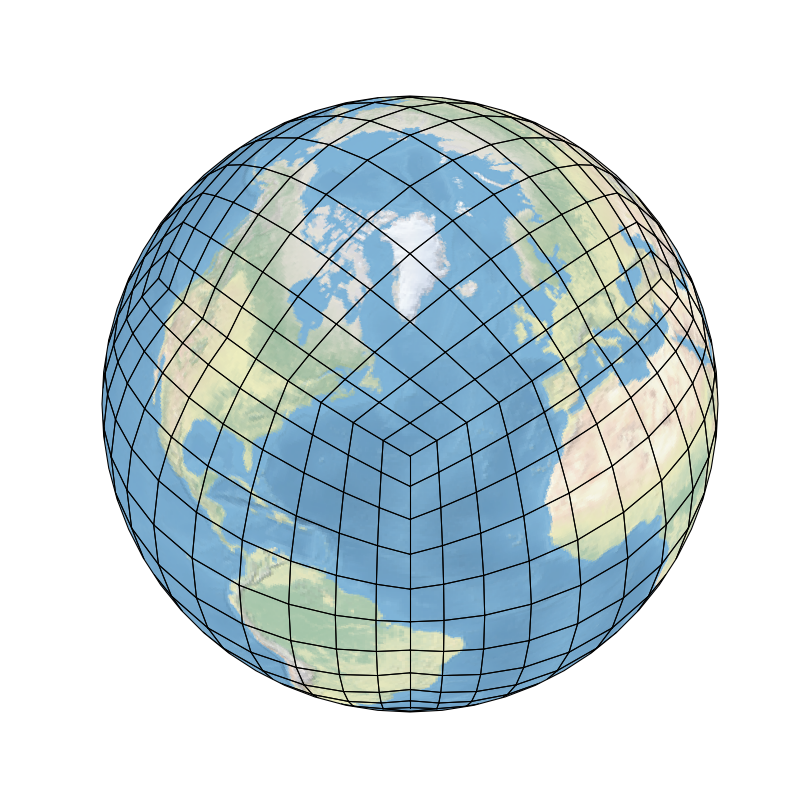
\includegraphics[width=1\linewidth]{gnomonic_equidistant_cs_10_sphere}
		\caption{Gridlines of the cube to the sphere mapping}
	\end{subfigure}
	\begin{subfigure}{0.42\textwidth}
		\centering
		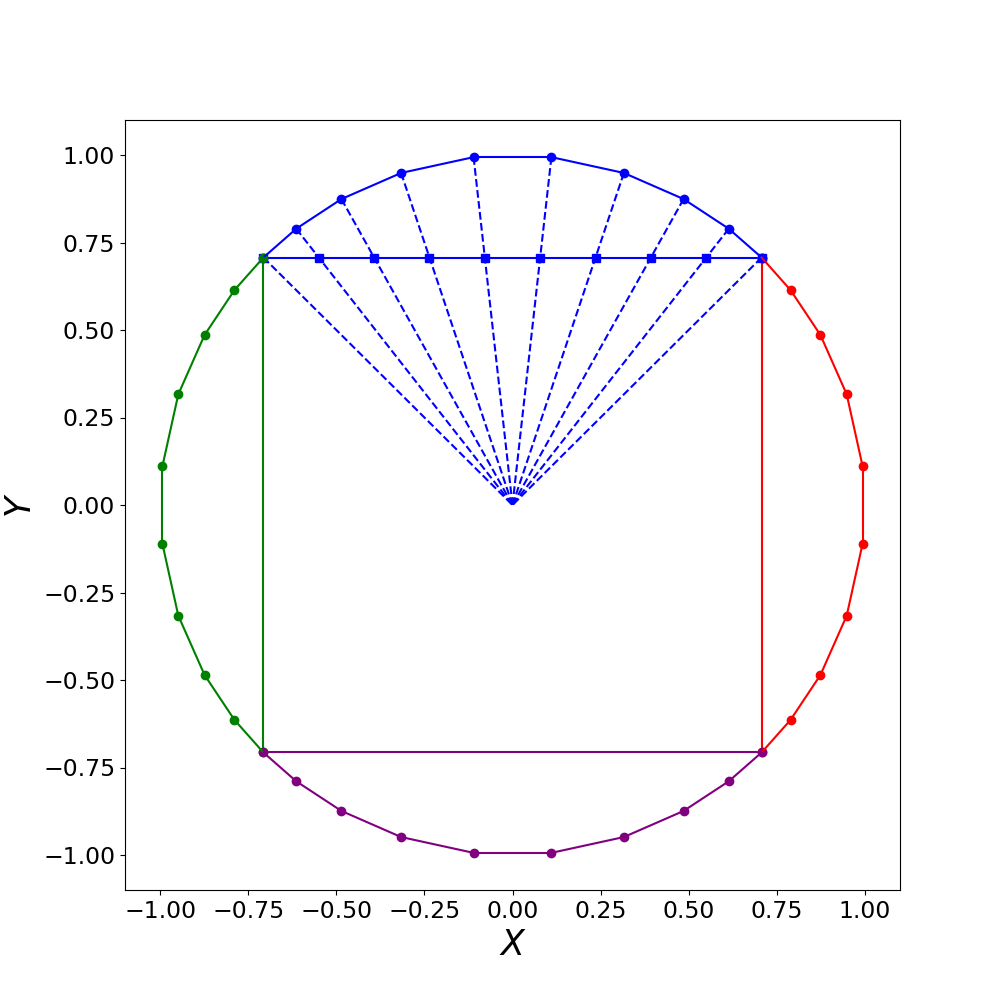
\includegraphics[width=1\linewidth]{g1}
		\caption{Cube and sphere mapping for $Z=0$.}
	\end{subfigure}
	\caption{(a) Illustration of the resulting cube-to-sphere mapping and (b) illustration of the cube-to-sphere projection.\label{chp-cs-equidistant}}
\end{figure}
The set of 6 maps $\{\boldsymbol{\Psi}_{p}, p = 1, \ldots, 6\}$ allow us to cover the sphere (Figure \ref{chp-cs-equidistant}).
Here $p$ denotes a panel, and they are defined and orientated as Figure \ref{chp-cs-panels}
shows. Then, we can represent a point on the sphere using the cubed-sphere coordinates
$(x,y,p)$.

\begin{figure}[!htb]
	\centering
	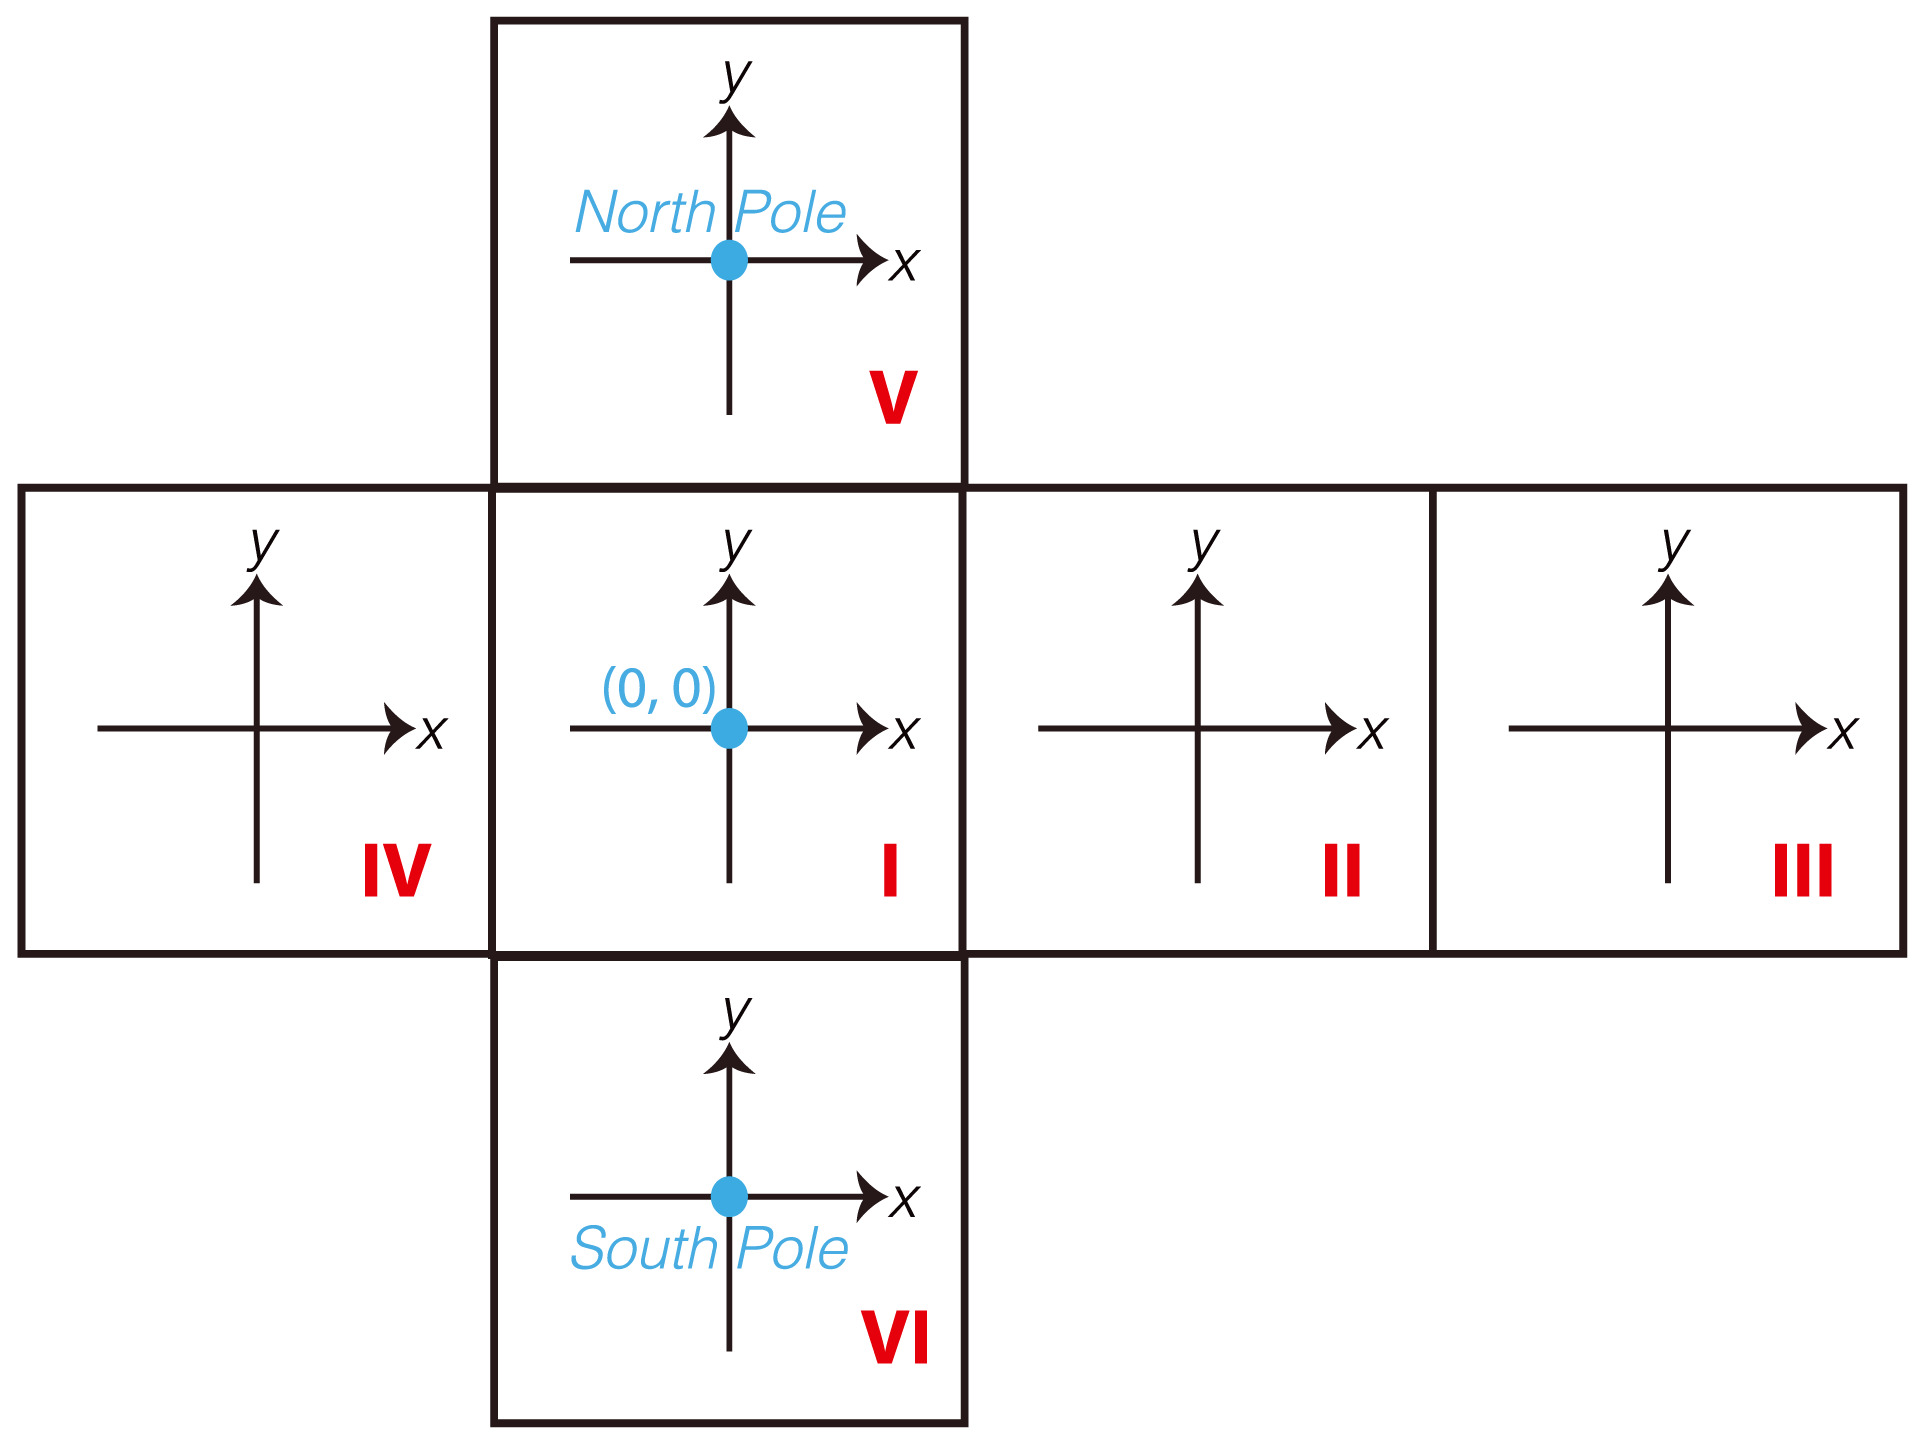
\includegraphics[width=0.4\linewidth]{chp4_panels}
	\caption{Cubed-sphere panels definition and orientation.
    Figure taken from \citet{jung:2019}.\label{chp-cs-panels}}
\end{figure}

The derivative of the maps $\boldsymbol{\Psi}_p$ are given by:
\begin{equation*}
	d\boldsymbol{\Psi}_{1}(x,y) = \frac{R}{{(1 + x^2 + y^2)}^{3/2}}
	\begin{bmatrix}
		-x & -y \\
	 	 1+y^2  & -xy \\
		 -xy  & 1+x^2
	\end{bmatrix},
\end{equation*}
\begin{equation*}
	d\boldsymbol{\Psi}_{2}(x,y) = \frac{R}{{(1 + x^2 + y^2)}^{3/2}}
	\begin{bmatrix}
		-(1+y^2) & xy \\
		 -x &  -y \\
		 -xy &  1+x^2
	\end{bmatrix},
\end{equation*}
\begin{equation*}
	d\boldsymbol{\Psi}_{3}(x,y) = \frac{R}{{(1 + x^2 + y^2)}^{3/2}}
	\begin{bmatrix}
		 x &  y \\
		-(1+y^2) & xy \\
		 -xy &  1+x^2
	\end{bmatrix},
\end{equation*}
\begin{equation*}
	d\boldsymbol{\Psi}_{4}(x,y) = \frac{R}{{(1 + x^2 + y^2)}^{3/2}}	
	\begin{bmatrix}
		 1+y^2 &  -xy \\
		 x & y \\
		 -xy &  1+x^2
	\end{bmatrix},
\end{equation*}
\begin{equation*}
	d\boldsymbol{\Psi}_{5}(x,y) = \frac{R}{{(1 + x^2 + y^2)}^{3/2}}	
	\begin{bmatrix}
		 xy  & -(1+x^2) \\
	 	 1+y^2  &  -xy \\
		-x & -y
	\end{bmatrix},
\end{equation*}
\begin{equation*}
	d\boldsymbol{\Psi}_{6}(x,y) = \frac{R}{{(1 + x^2 + y^2)}^{3/2}}
	\begin{bmatrix}
		 -xy  &  1+x^2 \\
		 1+y^2  &  -xy \\
		 x &  y
	\end{bmatrix}.
\end{equation*}
With the aid of the derivative, we may define a basis of tangent vectors 
$\{{\partial_x \boldsymbol{\Psi}},  {\partial_y \boldsymbol{\Psi}}\}$ on each point on the sphere by:
\begin{equation*}
	{\partial_x \boldsymbol{\boldsymbol{\Psi}}}(x,y,p) = d\boldsymbol{\boldsymbol{\Psi}}_{p}(x,y) \cdot
	\begin{bmatrix}
		 1 \\
		 0
	\end{bmatrix}, \quad
	{\partial_y \boldsymbol{\boldsymbol{\Psi}}}(x,y,p) = d\boldsymbol{\boldsymbol{\Psi}}_{p}(x,y) \cdot
	\begin{bmatrix}
		 0 \\
		 1
	\end{bmatrix}.
\end{equation*}
Notice that the matrix
\begin{equation*}
	\label{chp-cs-eqdistant-Psitensor}
	G_{\boldsymbol{\Psi}}(x,y) := 
	[d\boldsymbol{\Psi}_{p}(x,y)]^Td\boldsymbol{\Psi}_{p}(x,y)
	= \frac{R^2}{(1 + x^2 + y^2)^2}
	\begin{bmatrix}
		  1+ x^2 &  -xy \\
		 -xy & 1 + y^2
	\end{bmatrix},
\end{equation*}
does not depend on $p$.
This matrix is known as metric tensor.
It is easy to see that:
\begin{equation}
	\label{chp-cs-eqdistant-Psi-metric-tensor}
	G_{\boldsymbol{\Psi}}(x,y) = 
	\begin{bmatrix}
		\langle  {\partial_x \boldsymbol{\Psi}_p}, {\partial_x  \boldsymbol{\Psi}_p} \rangle & 
		\langle  {\partial_x \boldsymbol{\Psi}_p}, {\partial_y  \boldsymbol{\Psi}_p} \rangle \\
		\langle  {\partial_x  \boldsymbol{\Psi}_p}, {\partial_y  \boldsymbol{\Psi}_p} \rangle  &
		\langle  {\partial_y  \boldsymbol{\Psi}_p}, {\partial_y  \boldsymbol{\Psi}_p} \rangle 
	\end{bmatrix},
\end{equation}
where $\langle \cdot, \cdot \rangle$ denotes 
the standard inner product of $\mathbb{R}^3$,
and that $G_{\Psi}(x,y)$ is positive-definite, 
$\forall (x,y) \in [-1,1]\times[-1,1]$.
The Jacobian of the metric tensor $G_{\boldsymbol{\Psi}}(x,y)$, denoted by $\sqrt{\mathfrak{g}_{\boldsymbol{\Psi}}}$ and called metric term, is then given by:
\begin{equation*}
        \sqrt{\mathfrak{g}_{\boldsymbol{\Psi}}}(x,y) :=
	\sqrt{|\det{G_{\boldsymbol{\Psi}}(x,y)}|} = \frac{R^2}{(1+x^2+y^2)^{3/2}}.
\end{equation*}
Now let us assume that we have a function $\beta:[-\alpha,\alpha] \to [-1,1]$, for some positive $\alpha>0$,
supposed to be bijective and $\mathcal{C}^1$ with inverse $\mathcal{C}^1$ as well.
That is, $\beta$ is a change of coordinates.
Let us consider $ \boldsymbol{\Phi}_p: [-\alpha,\alpha]\times [-\alpha,\alpha] \to \mathbb{S}^2_R$,
given by 
\begin{equation*}
	\boldsymbol{\Phi}_p(x,y) := \boldsymbol{\Psi}_p\big(\beta(x),\beta(y)\big).
\end{equation*}
It follows from the chain rule that:
\begin{equation*}
        d \boldsymbol{\Phi}_p(x,y) = d \boldsymbol{\Psi}_p\big(\beta(x),\beta(y)\big)\cdot\text{diag}\big(\beta'(x),\beta'(y)\big),
\end{equation*}
where $\text{diag}(\beta'(x),\beta'(y))$ is a diagonal $2\times 2$ matrix with diagonal entries given by $\beta'(x)$ and $\beta'(y)$.
We also have that tangent vector basis $\{{\partial_x  \boldsymbol{\Phi}_p},  {\partial_y  \boldsymbol{\Phi}_p}\}$ satisfying
\begin{align*}
	{\partial_x  \boldsymbol{\Phi}_p}(x,y) = \beta'(x) \cdot {\partial_x  \boldsymbol{\Psi}_p}\big(\beta(x),\beta(y)\big),\\
	{\partial_y  \boldsymbol{\Phi}_p}(x,y) = \beta'(y) \cdot {\partial_y  \boldsymbol{\Psi}_p}\big(\beta(x),\beta(y)\big).
\end{align*}
The metric tensor of $\boldsymbol{\Phi}_p$ is defined as $G_{\Psi}$ in Equation \eqref{chp-cs-eqdistant-Psi-metric-tensor}:
\begin{equation*}
	\label{chp-cs-eqdistant-Phi-metric-tensor}
	G(x,y) = 
	\begin{bmatrix}
		\langle  {\partial_x  \boldsymbol{\Phi}_p}, {\partial_x \boldsymbol{\Phi}_p} \rangle & 
		\langle  {\partial_x  \boldsymbol{\Phi}_p}, {\partial_y \boldsymbol{\Phi}_p} \rangle \\
		\langle  {\partial_x  \boldsymbol{\Phi}_p}, {\partial_y \boldsymbol{\Phi}_p} \rangle  &
		\langle  {\partial_y  \boldsymbol{\Phi}_p}, {\partial_y \boldsymbol{\Phi}_p} \rangle 
	\end{bmatrix}.
\end{equation*}
Finally, the metric term $\sqrt{\mathfrak{g}}:= \sqrt{\det{G}}$ is expressed in terms of $\sqrt{\mathfrak{g}}_{\Psi}$ as
\begin{align*}
    \sqrt{\mathfrak{g}}(x,y) &= \beta'(x)\beta'(y)\sqrt{\mathfrak{g}}_{\Psi}\big(\beta(x),\beta(y)\big)\\
    &= \beta'(x)\beta'(y)\frac{R^2}{\big(1+\beta(x)^2+\beta(y)^2\big)^{3/2}}.
\end{align*}

\newpage
\section{Cubed-sphere grids}
\label{sec-cs-grids}
Now that we have established between the mapping between the cube and sphere with coordinate changes,
we may introduce the cubed-sphere grids proposed in the literature.

\subsection{Equidistant cubed-sphere}
\label{cs-equidistant}
The first cubed-sphere grid was proposed by \citet{sadourny:1972}. This grid is obtained by using
$\beta(x) = x$, $\alpha=1$ in the $\boldsymbol{\Phi}_p$ mapping described in Section \ref{equidistant-cs}.
This grid partitions the cube face into equally spaced points
and projects them onto the sphere, as illustrated in Figure
\ref{chp-cs-equidistant}, hence the name equidistant.
We shall denote this grid by \textbf{g1} since the parameter
\textbf{grid\_type} in FV3 is set equal to 1 to use this grid.

\subsection{Equiangular cubed-sphere}
\label{cs-equiangular}
Another cubed-sphere mapping is the equiangular mapping, 
introduced by \citet{ronchi:1996}, which leads to a more uniform grid.
This grid is obtained by considering the mapping $\boldsymbol{\Phi}_p$ described in Section \ref{equidistant-cs}
with $\beta(x) = \tan{x}$ and $\alpha=\frac{\pi}{4}$.
In this case, $\beta(x)$ represents the angular coordinates, and the cube-sphere is obtained by partitioning the angle between
grid points equally, as illustrated in Figure \ref{chp-cs-equiangular}, hence the name equiangular.
This grid is denoted by \textbf{g2}, for the same reason of the notation \textbf{g1}.
\begin{figure}[!htb]
	\centering
	\begin{subfigure}{0.42\textwidth}
		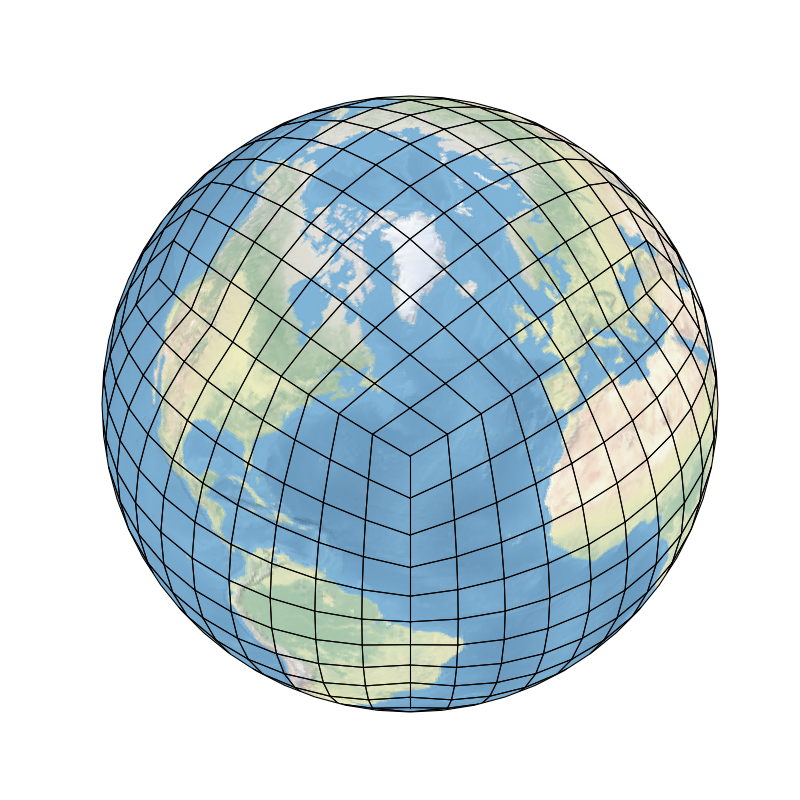
\includegraphics[width=1\linewidth]{gnomonic_equiangular_cs_10_sphere}
		\caption{Gridlines of the cube to the sphere equiangular mapping}
	\end{subfigure}
	\begin{subfigure}{0.42\textwidth}
		\centering
		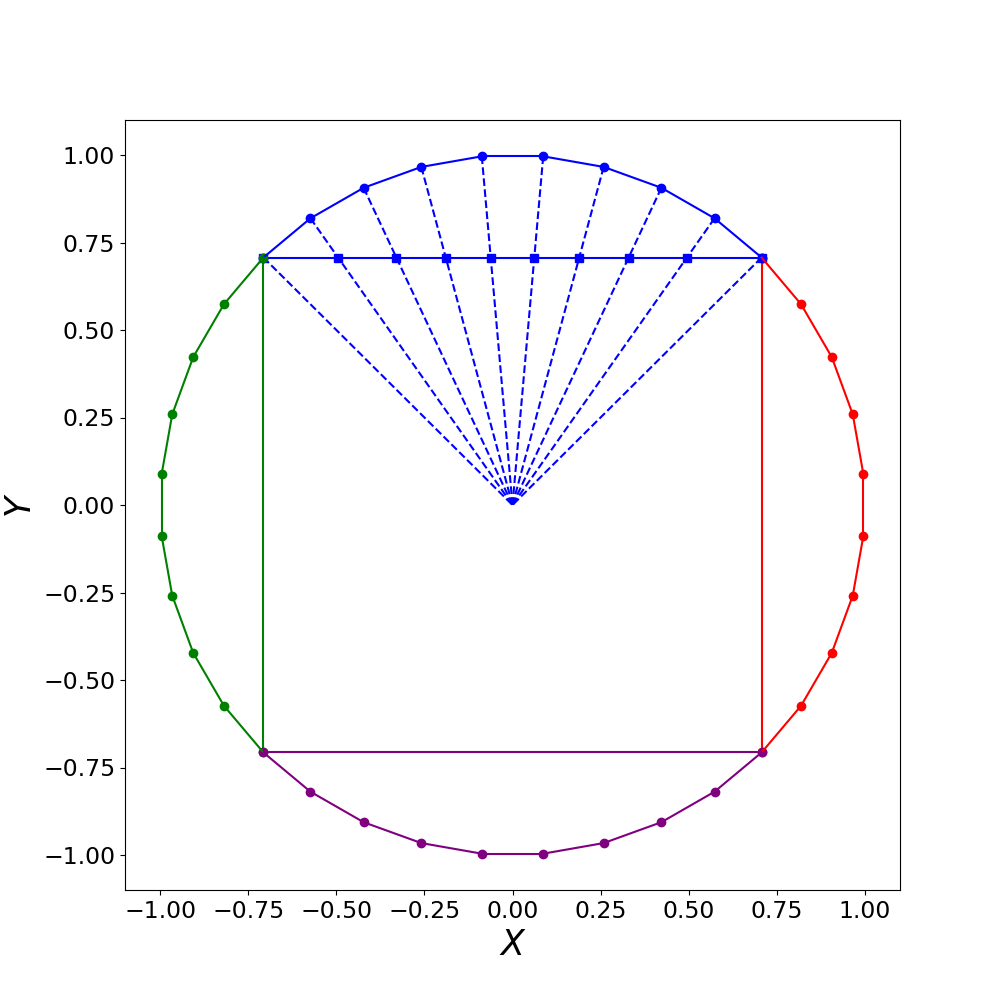
\includegraphics[width=1\linewidth]{g2}
		\caption{Cube and sphere equiangular mapping for $Z=0$.}
	\end{subfigure}
	\caption{(a) Illustration of the resulting cube-to-sphere mapping and (b) illustration of the cube-to-sphere projection using the equiangular mapping.\label{chp-cs-equiangular}}
\end{figure}

\subsection{Equi-edge cubed-sphere}
\label{cs-equiedge}
An equiangular cubed-sphere modification 
\citet{chen:2021} by using $\beta(x) = \sqrt{2}\tan{x}$ and
$\alpha=\arcsin{\big(\frac{1}{\sqrt{3}}\big)}$.
Figure \ref{chp-cs-equiedge} illustrates the equi-edge mapping.
\begin{figure}[!htb]
	\centering
	\begin{subfigure}{0.42\textwidth}
		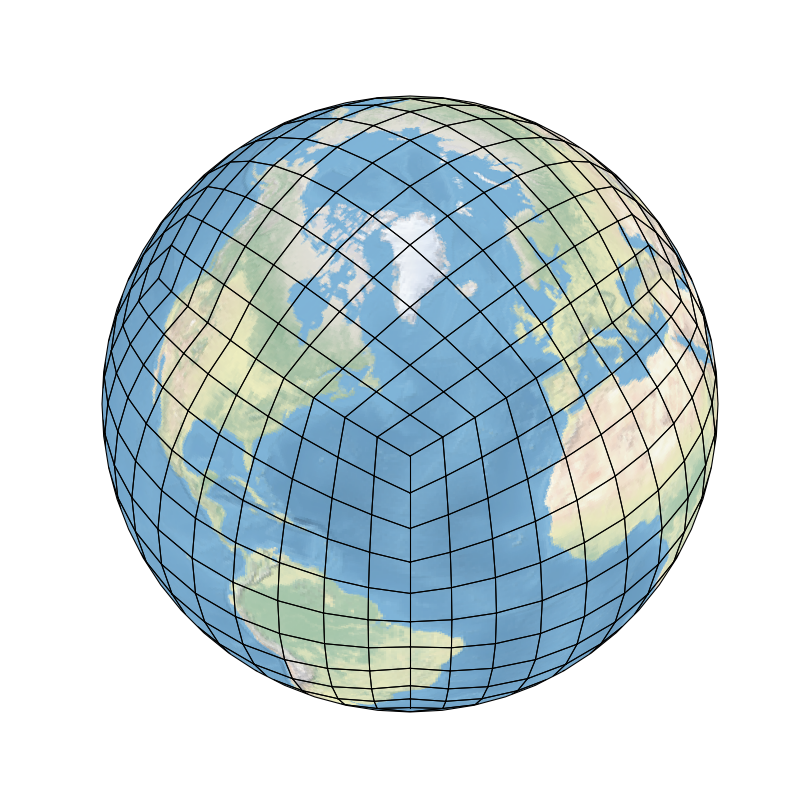
\includegraphics[width=1\linewidth]{gnomonic_equiedge_cs_10_sphere}
		\caption{Gridlines of the cube to the sphere equi-edge mapping}
	\end{subfigure}
	\begin{subfigure}{0.42\textwidth}
		\centering
		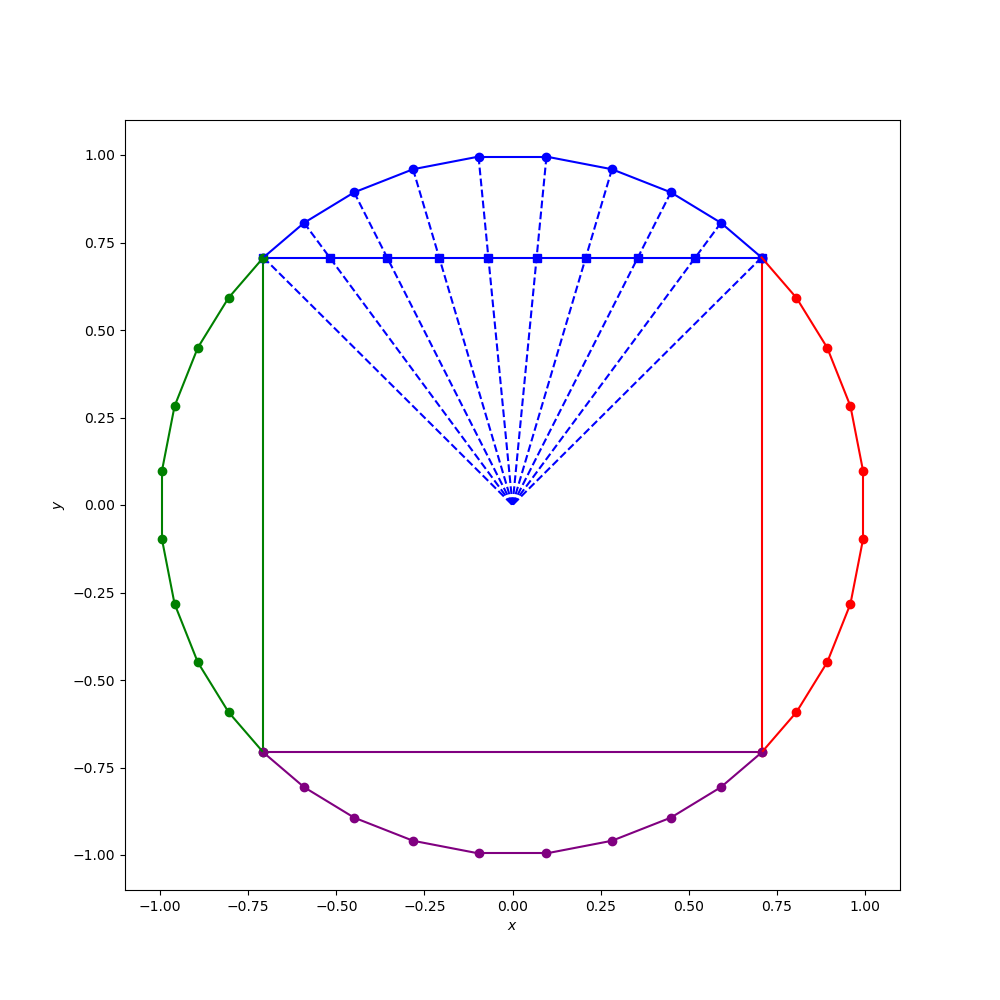
\includegraphics[width=1\linewidth]{g0}
		\caption{Cube and sphere equi-edge mapping for $Z=0$.}
	\end{subfigure}
	\caption{(a) Illustration of the resulting cube-to-sphere mapping and (b) illustration of the cube-to-sphere projection using the equi-edge mapping.\label{chp-cs-equiedge}}
\end{figure}

The idea behind the equi-edge cubed-sphere lies in partitioning the edges of the spherical cube equally,
and then generating the other cells, hence the name equi-edge.
This grid is denoted by \textbf{g0}, for the same reason of the notation \textbf{g1}.
Also, this grid leads to more uniform cells after applying the grid stretching option of FV3 \citep{harris:2016, chen:2021}.

\subsection{Geometric properties}
We will utilize the notation introduced in Section \ref{chp-adv2d-sec-not} throughout this Chapter.
We shall used the earth radius $R = 6.371 \times 10^6$ meters.
The parameter $\nu$ represents a non-negative integer indicating the number of ghost cell layers in each panel boundary, called halo size.
To generate the cubed-sphere, we consider a $(\Delta x, \Delta y)$-grid denoted by 
$\Omega_{\Delta x, \Delta y} = (\Omega_{ij})_{i,j=-\nu+1,\ldots,N+\nu}$, 
where $\Delta x = \Delta y$, and it covers the domain $\Omega$. 
A control volume of the cubed-sphere is denoted by $\Omega_{ijp}$, defined as follows:
\begin{equation*}
	\Omega_{ijp} = \Phi_p(\Omega_{ij})
	\quad -\nu+1 \leq i, j \leq N+\nu, \quad 1 \leq p \leq 6.
\end{equation*}
The cubed-sphere grid refers to the collection of control volumes 
$(\Omega_{ijp})_{i,j=-\nu+1,\ldots,N+\nu}^{p=1,\ldots,6}$. 
In Figures \ref{chp-cs-equidistant}, \ref{chp-cs-equiangular} and \ref{chp-cs-equiedge} examples of the cubed-sphere grids are depicted,
excluding the ghost cells.
These grids are generated using the equidistant, equiangular and equi-edge mappings for $N=10$.

We will denote the area of $\Omega_{ijp}$ by $|\Omega_{ij}|$.
Notice that the area does not depend on the panel due to the grid symmetry.
We also define the diameter of a cell as $2\sqrt{\frac{|\Omega_{ij}|}{\pi}}$, which corresponds to the diameter of a circle with area $|\Omega_{ij}|$.
The control volume area is given by:
\begin{equation}
	\label{chp4-area}
	|\Omega_{ij}| = \int_{x_{i-\frac{1}{2}}}^{x_{i+\frac{1}{2}}} \int_{y_{j-\frac{1}{2}}}^{y_{j+\frac{1}{2}}}{\sqrt{\mathfrak{g}}(x,y)} \,dx \,dy = 
	|\hat{\Omega}_{ij}| + \mathcal{O}(\Delta x^2),
\end{equation}
where $|\hat{\Omega}_{ij}| = \sqrt{\mathfrak{g}}(x_i,y_j) \Delta x \Delta y$,
and the last equality follows from Proposition \ref{prop-bound-centroid-2d}.
In tables \ref{g0-dx-table}, \ref{g1-dx-table}, and \ref{g2-dx-table},
we display the diameters of the grids g0, g1, and g2 for $N=48\times 2^k$, 
where $k = 0,\ldots, 4$. These values of $N$ are considered in this work.
Similarly, in tables \ref{g0-da-table}, \ref{g1-da-table}, and \ref{g2-da-table}, we display the areas.


\begin{table}[htbp]
    \centering
    \caption{Mean diameter, minimum diameter, and maximum diameter for different values of $N$ considering the equi-edge grid (g0).\label{g0-dx-table}}
    \begin{tabular}{cccccc}
        \toprule
        $N$ & Mean Length (km) & Min Length (km) & Max Length (km) & $\frac{\text{Max}}{\text{Min}}$ \\
        \midrule
        48 & 218 & 175 & 266 & 1.5192 \\
        96 & 108 & 86 & 131 & 1.5195 \\
        192 & 54 & 43 & 65 & 1.5196 \\
        384 & 26 & 21 & 32 & 1.5197 \\
        768 & 13 & 10 & 16 & 1.5197 \\
        \bottomrule
    \end{tabular}
\end{table}

\begin{table}[htbp]
    \centering
    \caption{As Table \ref{g0-dx-table} but considering the equidistant grid (g1). \label{g1-dx-table}}
    \begin{tabular}{cccccc}
        \toprule
        $N$ & Mean Length (km) & Min Length (km) & Max Length (km) & $\frac{\text{Max}}{\text{Min}}$ \\
        \midrule
        48 & 215 & 134 & 305 & 2.2780 \\
        96 & 107 & 66 & 151 & 2.2791 \\
        192 & 53 & 33 & 75 & 2.2794 \\
        384 & 26 & 16 & 37 & 2.2795 \\
        768 & 13 & 8 & 18 & 2.2795 \\
        \bottomrule
    \end{tabular}
\end{table}

\begin{table}[htbp]
    \centering
    \caption{As Table \ref{g0-dx-table} but considering the equiangular grid (g2). \label{g2-dx-table}}
    \begin{tabular}{cccccc}
        \toprule
        $N$ & Mean Length (km) & Min Length (km) & Max Length (km) & $\frac{\text{Max}}{\text{Min}}$ \\
        \midrule
        48 & 220 & 202 & 240 & 1.1890 \\
        96 & 109 & 99 & 118  & 1.1892 \\
        192 & 54 & 49 & 59  & 1.1892 \\
        384 & 27 & 24 & 29  & 1.1892 \\
        768 & 13 & 12 & 14  & 1.1892 \\
        \bottomrule
    \end{tabular}
\end{table}


\begin{table}[htbp]
    \centering
    \caption{Mean area, minimum area, and maximum area for different values of $N$ considering the equi-edge grid (g0).\label{g0-da-table}}
    \begin{tabular}{cccccc}
        \toprule
        $N$ & Mean Area (km$^2$) & Min Area (km$^2$) & Max Area (km$^2$) & $\frac{\text{Max}}{\text{Min}}$ \\
        \midrule
        48 & 38033 & 24113 & 55650 & 2.3078 \\
        96 & 9364 & 5902 & 13628 & 2.3090 \\
        192 & 2323 & 1460 & 3371 & 2.3093 \\
        384 & 578 & 363 & 838 & 2.3094 \\
        768 & 144 & 90 & 209 & 2.3094 \\
        \bottomrule
    \end{tabular}
\end{table}

\begin{table}[htbp]
    \centering
    \caption{As Table \ref{g0-da-table} but considering the equidistant grid (g1). \label{g1-da-table}}
    \begin{tabular}{cccccc}
        \toprule
        $N$ & Mean Area (km$^2$) & Min Area (km$^2$) & Max Area (km$^2$) & $\frac{\text{Max}}{\text{Min}}$ \\
        \midrule
        48 & 37762 & 14145 & 73403 & 5.1891 \\
        96 & 9331 & 3462 & 17985 & 5.1944 \\
        192 & 2319 & 856 & 4450 & 5.1957 \\
        384 & 578 & 213 & 1106 & 5.1960 \\
        768 & 144 & 53 & 276 & 5.1961 \\
        \bottomrule
    \end{tabular}
\end{table}

\begin{table}[htbp]
    \centering
    \caption{As Table \ref{g0-da-table} but considering the equiangular grid (g2). \label{g2-da-table}}
    \begin{tabular}{cccccc}
        \toprule
        $N$ & Mean Area (km$^2$) & Min Area (km$^2$) & Max Area (km$^2$) & $\frac{\text{Max}}{\text{Min}}$ \\
        \midrule
        48 & 38269 & 32062 & 45327 & 1.4137 \\
        96 & 9393 & 7847 & 11096 & 1.4141 \\
        192 & 2327 & 1941 & 2745 & 1.4142 \\
        384 & 579 & 482 & 682 & 1.4142 \\
        768 & 144 & 120 & 170 & 1.4142 \\
        \bottomrule
    \end{tabular}
\end{table}


We can observe that in terms of areas and diameters of the cells, grid g1 is the least uniform,
while g2 is the most uniform grid.
Grid g0 is more uniform than g1, but the maximum/minimum ratio of the areas is almost 2.3. 
Despite this, g0 is operational in some applications of FV3 \citep{harris:2021,chen:2021}, such as, for instance, 
the Next Generation Global Prediction System (NGGPS) \citep{zhou:2019}, 
because this grid is expected to produce less grid imprinting due to its greater uniformity near the cubed edges.
Therefore, in this thesis, we shall constrain our attention only to grids g0 and g2, since g2 is ideally more uniform and g0 is currently used in FV3.
In Figure \ref{chp-cs-areas}, we illustrate the areas of both grids, g0 and g2.
We can observe that the areas of g0 exhibit a higher gradient near the cube corners, while g2 appears to have a higher gradient near the middle of the cube edges.
\begin{figure}[!htb]
	\centering
	\begin{subfigure}{0.48\textwidth}
		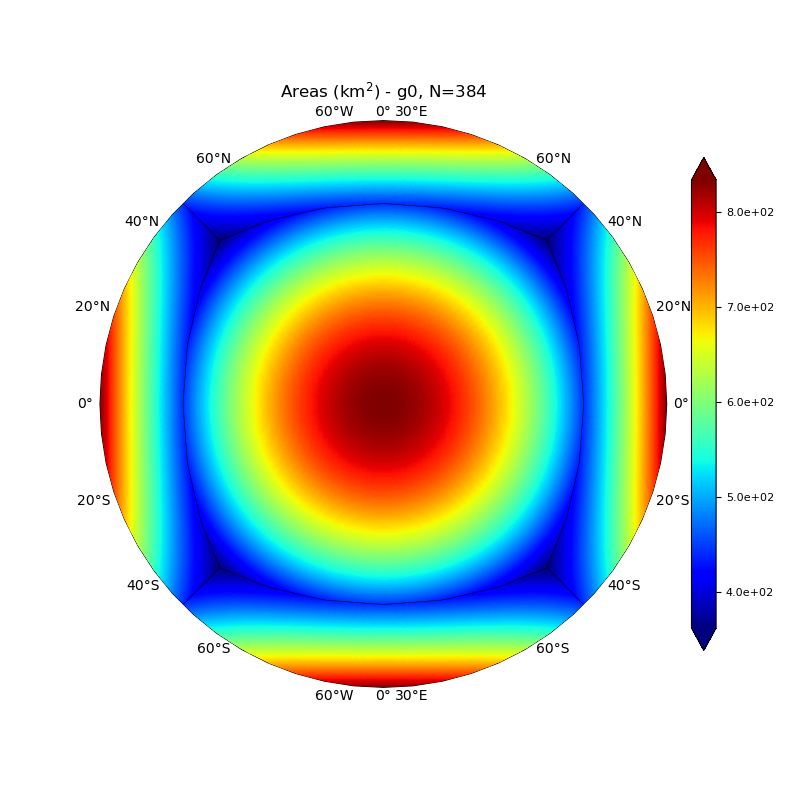
\includegraphics[width=0.8\linewidth]{g0_384}
		\caption{g0 grid areas (km$^2$).}
	\end{subfigure}
	\begin{subfigure}{0.48\textwidth}
		\centering
		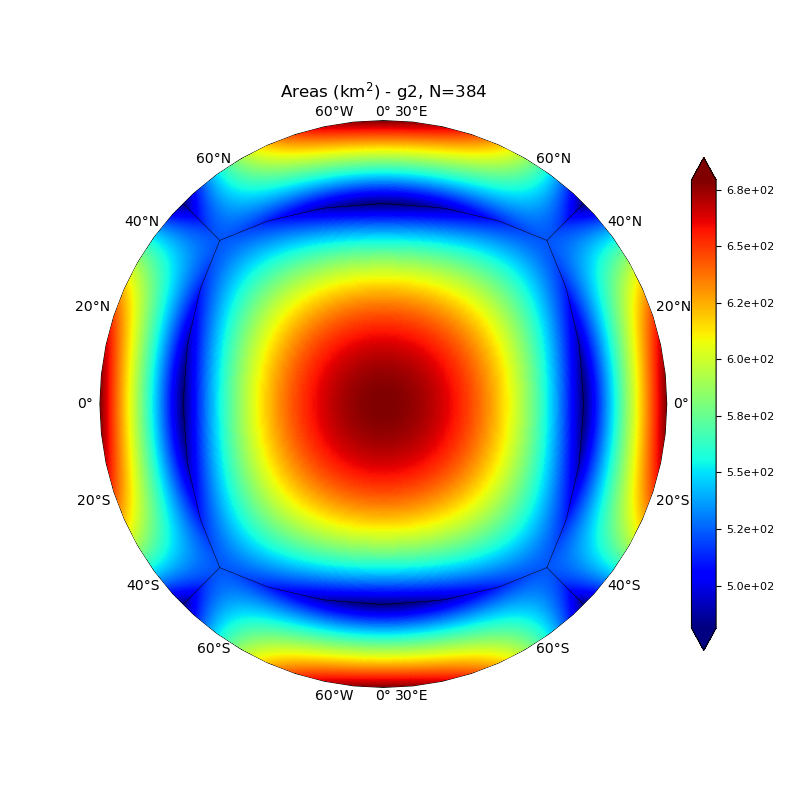
\includegraphics[width=0.8\linewidth]{g2_384}
		\caption{g2 grid areas (km$^2$).}
	\end{subfigure}
	\caption{Areas for the grid g0 and g2 using $N=384$.\label{chp-cs-areas}}
\end{figure}

There are four types of grid points on the cubed-sphere that we need to compute: the A-grid, B-grid, C-grid, and D-grid points.
These names are based on the Arakawa grids \citep{arakawa:1977}.
The locations of these points are illustrated in Figure \ref{chp-cs-gridpoints} for the g2 grid.
\begin{figure}[!htb]
	\centering
	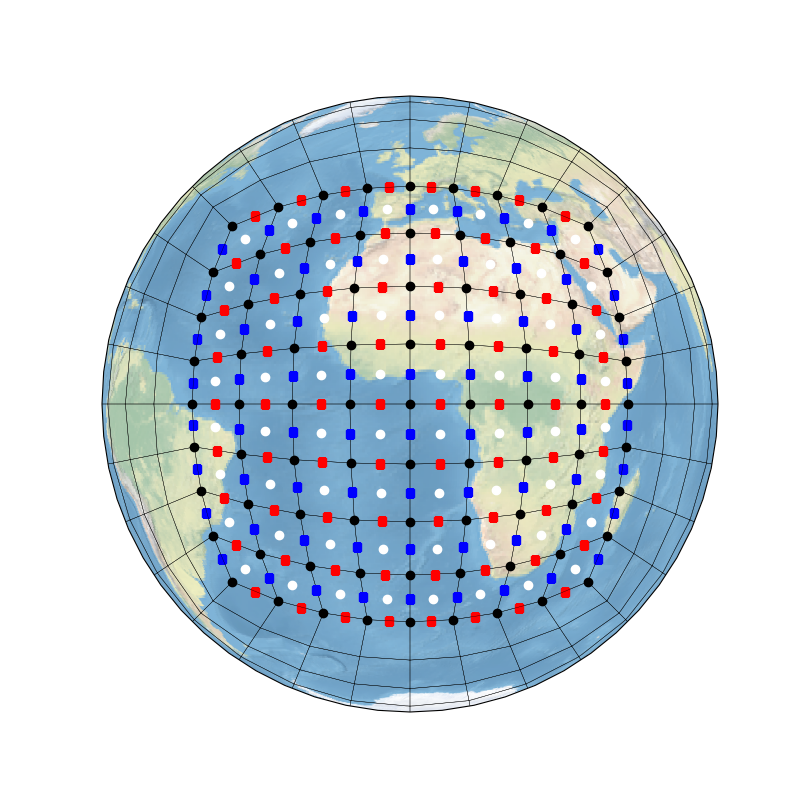
\includegraphics[width=0.5\linewidth]{gridpoints_sphere}
	\caption{Illustration of the A-grid (white) B-grid (black), C-grid (blue) and D-grid (red) points 
		for the g2 grid with $N=10$.\label{chp-cs-gridpoints}}
\end{figure}

One possible approach is to use the cubed-sphere mapping to generate these points, based on the grid points projected onto the sphere from the plane.
These points shall be denoted using a superscript 'c'.
The B-grid points represent the corners of the control volume, namely
\begin{equation}
	\Phi_{i+\frac{1}{2},j+\frac{1}{2},p}^c := \Phi_p(x_{i+\frac{1}{2}},y_{j+\frac{1}{2}}).
\end{equation}
Similarly, the A grid points are the cell centers:
\begin{equation}
	\Phi_{ijp}^c := \Phi_p(x_{i},y_{j}).
\end{equation}
The C-grid points are the midpoints of the edge in the $y$-direction, namely:
\begin{equation}
	\Phi_{i+\frac{1}{2},j,p}^c := \Phi_p(x_{i+\frac{1}{2}},y_{j}).
\end{equation}
The D-grid points are the midpoints of the edge in the $x$-direction, namely:
\begin{equation}
	\Phi_{i,j+\frac{1}{2},p}^c := \Phi_p(x_{i},y_{j+\frac{1}{2}}).
\end{equation}
The grids g0 and g2, formulated with these grid points, are denoted by \textbf{g0.c} and \textbf{g2.c}, respectively.
We refer to this grid point formulation as cube midpoints, which is a common approach used in the literature \citep{guo:2014,katta:2015,katta:2015b,nair:2005,ullrich:2016}.

Another way to compute the grid points, which is used in FV3, is to compute the B-grid
points using as before and obtain the A, C and D-grids using the spherical midpoints.
These points shall be denoted using a superscript 's'.
The B-grid points in this case are:
\begin{equation}
	\Phi_{i+\frac{1}{2},j+\frac{1}{2},p}^s := \Phi_{i+\frac{1}{2},j+\frac{1}{2},p}^c.
\end{equation}
The A-grid points are computed by averaging the values of 4 B-grid points:
\begin{equation}
	\Phi_{ijp}^s :=
	\frac{\Phi_{i+\frac{1}{2},j+\frac{1}{2},p}^s + \Phi_{i+\frac{1}{2},j-\frac{1}{2},p}^s + \Phi_{i-\frac{1}{2},j+\frac{1}{2},p}^s + \Phi_{i-\frac{1}{2},j-\frac{1}{2},p}^s}
         {\|\Phi_{i+\frac{1}{2},j+\frac{1}{2},p}^s + \Phi_{i+\frac{1}{2},j-\frac{1}{2},p}^s + \Phi_{i-\frac{1}{2},j+\frac{1}{2},p}^s + \Phi_{i-\frac{1}{2},j-\frac{1}{2},p}^s\|}.
\end{equation}
Similarly, the C-grid points are obtained by averaging the values of 2 B-grid points.
\begin{equation}
	\Phi_{i+\frac{1}{2},j,p}^s :=
	\frac{\Phi_{i+\frac{1}{2},j+\frac{1}{2},p}^s + \Phi_{i+\frac{1}{2},j-\frac{1}{2},p}^s}
	   {\|\Phi_{i+\frac{1}{2},j+\frac{1}{2},p}^s + \Phi_{i+\frac{1}{2},j-\frac{1}{2},p}^s\|}.
\end{equation}
and the D-grid points are also  given by the average  the values of 2 B-grid points:
\begin{equation}
	\Phi_{i,j+\frac{1}{2},p}^s :=
	\frac{\Phi_{i+\frac{1}{2},j+\frac{1}{2},p}^s + \Phi_{i-\frac{1}{2},j+\frac{1}{2},p}^s}
	     {\|\Phi_{i+\frac{1}{2},j+\frac{1}{2},p}^s + \Phi_{i-\frac{1}{2},j+\frac{1}{2},p}^s\|}.
\end{equation}
The grids g0 and g2, formulated with these grid points, are denoted by \textbf{g0.s} and \textbf{g2.s}, respectively.
We refer to this grid points formulation as spherical midpoints.
One can easily see that:
\begin{align}
	\Phi_{i+\frac{1}{2},j,p}^s &= \Phi_{i+\frac{1}{2},j,p}^c+ \mathcal{O}(\Delta x^2),\\
	\Phi_{i,j+\frac{1}{2},p}^s &= \Phi_{i,j+\frac{1}{2},p}^c+ \mathcal{O}(\Delta x^2),\\
	\Phi_{i,j,p}^s &= \Phi_{i,j,p}^c + \mathcal{O}(\Delta x^2).
\end{align}
Then, we should expect similar results when using different grid point formulations, especially when using a high-resolution grid.
In g0.c or g2.c grids, the points are aligned along geodesics.
This happens because the cube-mapping maps lines on the plane onto geodesics on the sphere.
However, one can see that this does not occur on g0.s or g2.s, as the A, C, and D-grid points are not aligned on the same geodesic.
Although this misalignment becomes negligible for high resolutions,
it impacts ghost cell interpolation accuracy, as we shall see in Section \ref{cs-halodata}.

Hereafter, we are going to omit the superscripts 's' and 'c'.
Finally, we introduce the following geodesic distances in $x$ and $y$ directions, respectively,
\begin{align}
	{\delta} x_{ij} &= d(\Phi_{i+\frac{1}{2},j,p},\Phi_{i-\frac{1}{2},j,p}) ,\\
	{\delta} y_{ij} &= d(\Phi_{i,j+\frac{1}{2},p},\Phi_{i,j-\frac{1}{2},p}),
\end{align}
where $d(P,Q) = R\arccos{(\langle P, Q \rangle)}$, for $P,Q \in \mathbb{S}^2_R$, and we assume that $i$ and $j$ can be integers or half-integers.
Notice that these distances do not depend on the panel due to the grid symmetry.
These distances may be represented in terms of the tangent vector norms as:
\begin{align}
	{\delta} x_{ij} &= 
	\int_{x_{i-\frac{1}{2}}}^{x_{i+\frac{1}{2}}}
	\|\partial_x  \mathbf{\Phi}_{p}\|(x,y_j) \,dx ,\\
	{\delta} y_{ij} &=
	\int_{y_{j-\frac{1}{2}}}^{y_{j+\frac{1}{2}}}
	\|\partial_y \mathbf{\Phi}_{p}\|(x_i,y) \,dy.
\end{align}
Hence, their midpoint approximations are defined as:
\begin{align}
	\hat{\delta} x_{ij} &= \|\partial_x \mathbf{\Phi}_{ijp} \|\Delta x,\\
	\hat{\delta} y_{ij} &= \|\partial_y \mathbf{\Phi}_{ijp} \|\Delta y,
\end{align}
which are second-order accurate (see Theorem \ref{prop-bound-midpoint1d}):
\begin{align}
\delta x_{ij} = \hat{\delta} x_{ij} + \mathcal{O}(\Delta x^2),\\
\delta y_{ij} = \hat{\delta} y_{ij} + \mathcal{O}(\Delta y^2).
\end{align}
\subsection{Duo-grid points}
\label{duogrid-points}
The B duo-grid points are generated by computing the mappings $\boldsymbol{\Phi}_p$ for the grid points 
$(x_{i+\frac{1}{2}}, y_{j+\frac{1}{2}})$ where $i$ and $j$ out of the range $0$ to $N$. 
When using the cube midpoint formulation, the A, C, and D-grid points are computed analogously.
In Figure \ref{cs-duo}, we illustrate the duo-grid points obtained for both g0 and g2 grids.
We can observe in Figure \ref{cs-duo-g2} that the B duo-grid points of g2 are aligned on common geodesics.
This property has been known since the work of \citet{ronchi:1996}, and similarly, it holds for A, C, and D duo-grid points when using the cube midpoint formulation.
This property is very useful because it allows us to use 1D Lagrange interpolation to estimate the duo-grid values using values 
from neighboring panels, and it has been widely used in the literature \citep{ross:2006, croisille:2013,katta:2015,katta:2015b, chen:2021}.

However, it is evident from Figure \ref{cs-duo-g0} that the analogous property does not hold for the g0 grid.
To address this problem, \citet{chen:2021} proposes modifying the ghost values of the $x$ and $y$ coordinates by mirroring certain points. 
This generates the new duo-grid points, aligning them on the same geodesic as those from the neighboring panel.
More formally, for $g=1,2,\ldots,\nu$, we introduce the mirrored values
\begin{align}
	\hat{x}_{-g+\frac{1}{2}}  &= \arctan\left(\frac{1}{\alpha}\tan\left(-\frac{\pi}{2}-\arctan{(\alpha \tan{x_{g+\frac{1}{2}} })}\right)\right),\\
	\hat{x}_{N+g+\frac{1}{2}} &= -\hat{x}_{-g+\frac{1}{2}}, \\
	\hat{y}_{-g+\frac{1}{2}}  &= \arctan\left(\frac{1}{\alpha}\tan\left(-\frac{\pi}{2}-\arctan{(\alpha \tan{y_{g+\frac{1}{2}} })}\right)\right),\\
	\hat{y}_{N+g+\frac{1}{2}} &= -\hat{y}_{-g+\frac{1}{2}},
\end{align}
to replace ${x}_{-g+\frac{1}{2}},{x}_{N+g+\frac{1}{2}},{y}_{-g+\frac{1}{2}}$ and ${y}_{N+g+\frac{1}{2}}$, respectively.
When computing the grid points using the cube midpoints formulation, the values of $x_i$ and $y_j$ are readjusted similarly.
Figure \ref{cs-duo-g02} illustrates how the modified duo-grid of g0 aligns with the geodesics of neighboring panels just as g2 (Figure \ref{cs-duo-g2}).
Notice, however, that the g0 B-grid will no longer be equally spaced in terms of its $x$ and $y$ coordinates,
in contrast to g2, where the $x$ and $y$ coordinates of the B-grid are uniformly spaced.
This may require special attention from numerical schemes using g0 near edges due to the loss of uniformity.
\begin{figure}[!htb]
	\centering
	\begin{subfigure}{0.45\textwidth}
		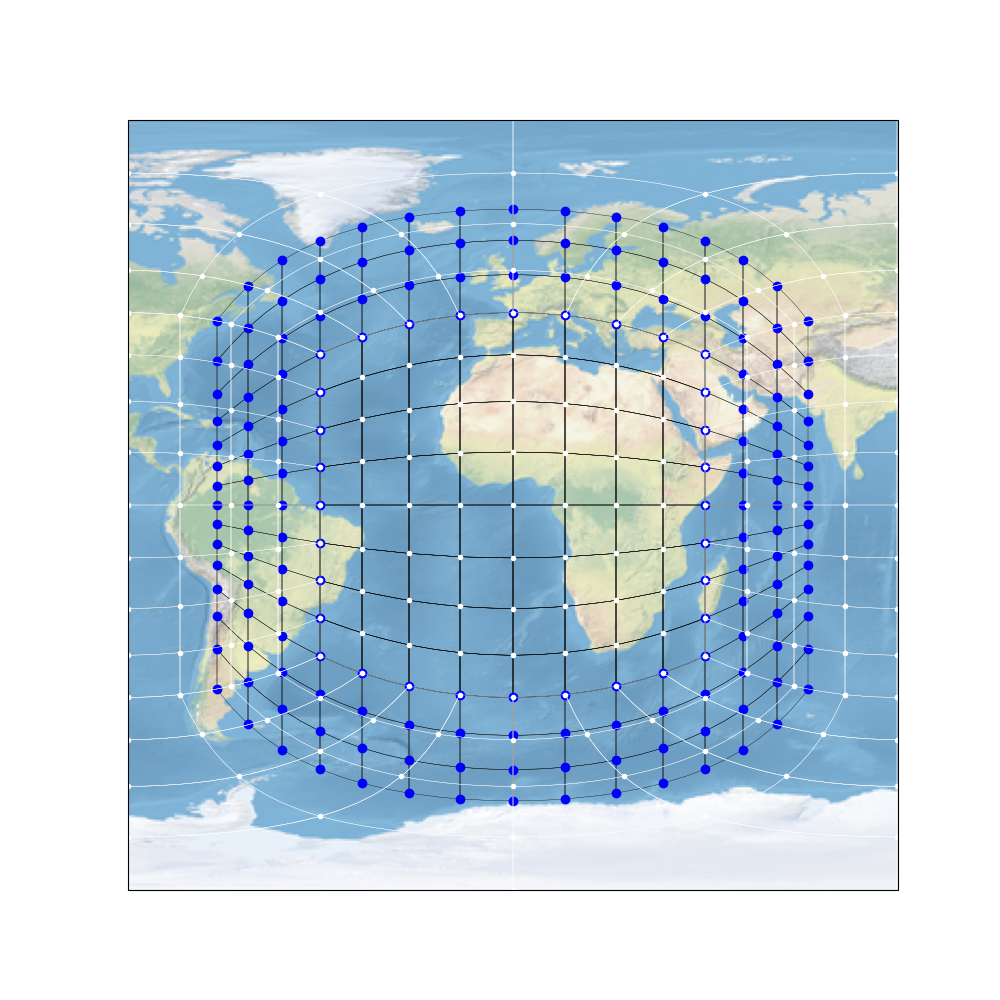
\includegraphics[width=1\linewidth]{g0_duo}
		\caption{g0 duo-grid.\label{cs-duo-g0}}
	\end{subfigure}
	\begin{subfigure}{0.45\textwidth}
		\centering
		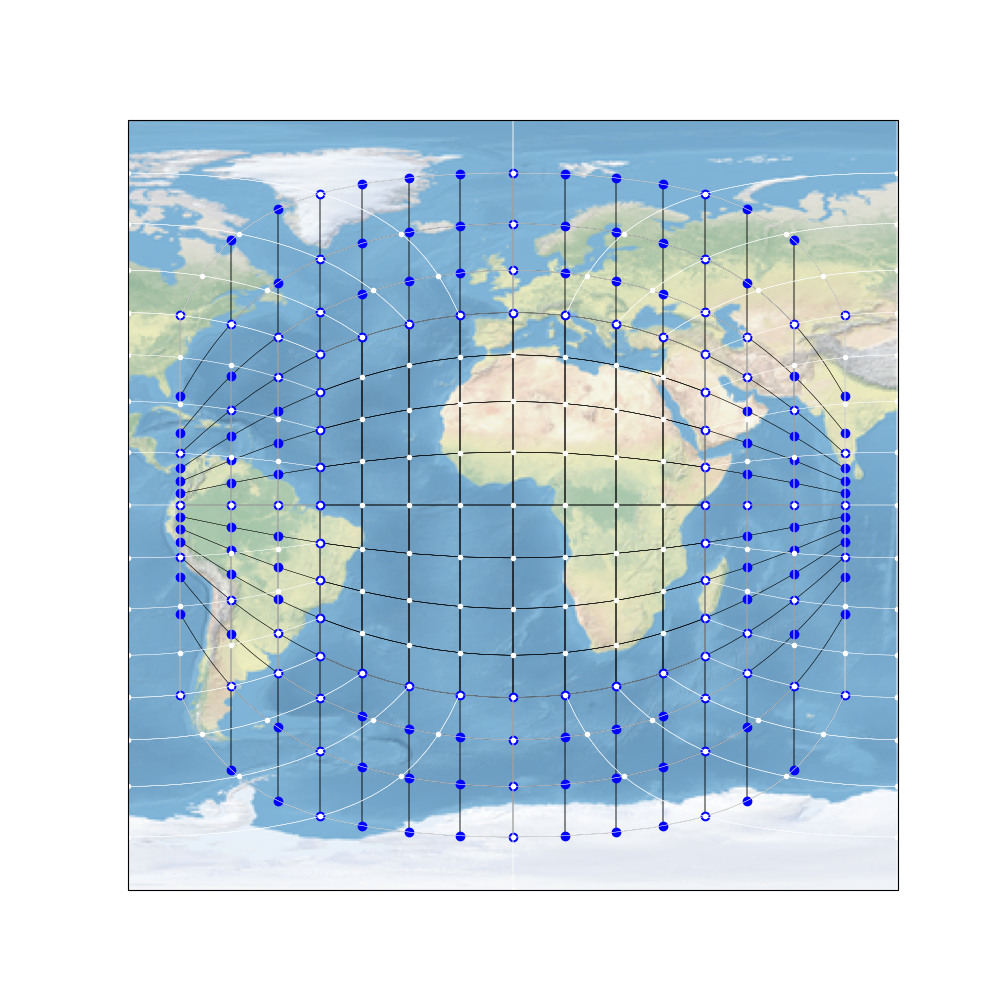
\includegraphics[width=1\linewidth]{g0_duo2}
		\caption{Mirrored g0 duo-grid.\label{cs-duo-g02}}
	\end{subfigure}
	\begin{subfigure}{0.45\textwidth}
		\centering
		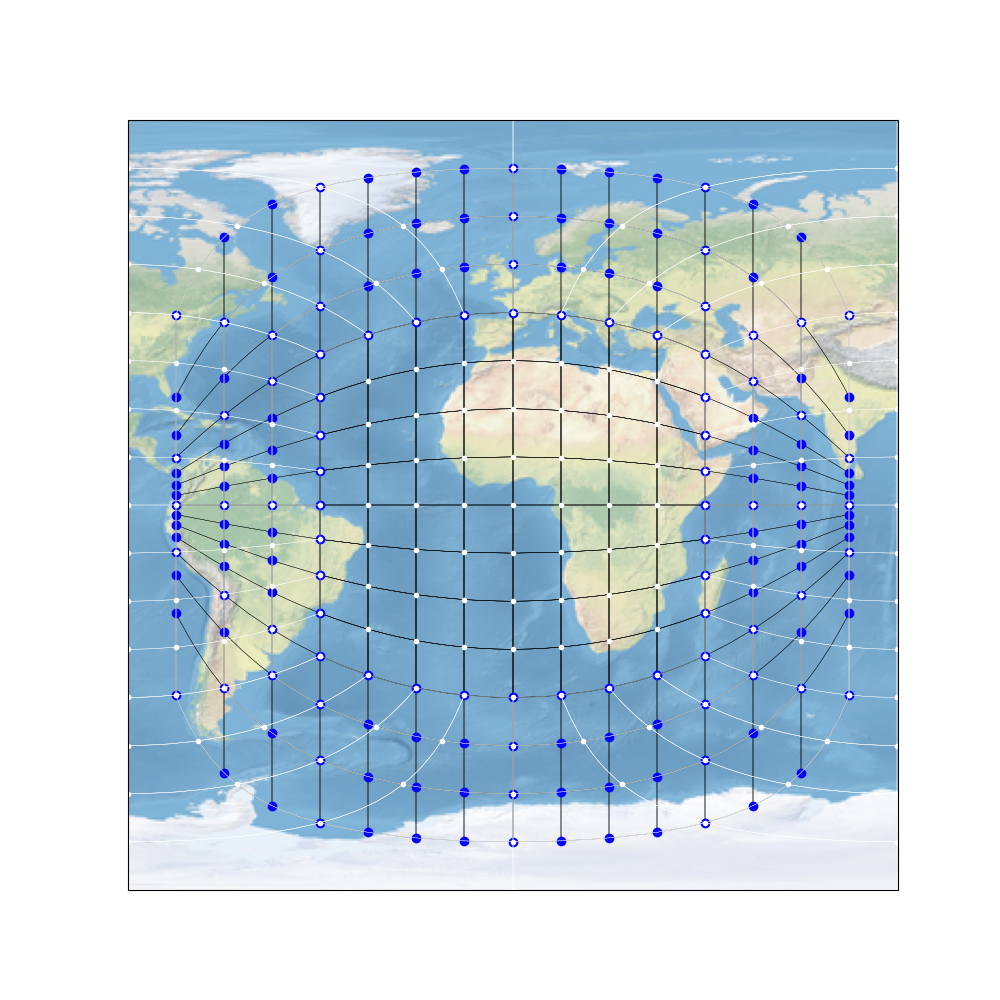
\includegraphics[width=1\linewidth]{g2_duo}
		\caption{g2 duo-grid.\label{cs-duo-g2}}
	\end{subfigure}
	\caption{Duo-grid lines of panel 1 for the g0 (a) and g2 (c). (b) shows the mirrored duo-grid of g0.
		B duo-grid points are denoted by blue circles, the B-grid points are denoted by white points.\label{cs-duo}}
\end{figure}

\subsection{Tangent vectors on the sphere}
\label{cs-tgvectors}
The tangent space at $P \in \mathbb{S}^2_R$ is denoted by $T_P \mathbb{S}^2$.
It is easy to see that:
\begin{equation*}
	T_P\mathbb{S}^2_R = \{P_0 \in \mathbb{R}^3: \langle P,P_0\rangle = 0\}.
\end{equation*}
We are going to consider three ways to represent an element of $\mathbb{S}_R^2$:
using $(X,Y,Z)$ coordinates, or using $(\lambda, \phi)$
latitude-longitude coordinates, or, at last, using the cubed-sphere
coordinates $(x,y,p)$, where $(x,y)$ are the cube face coordinates and 
$p \in \{1,2,\cdots, 6\}$ stands for a cube panel.
We say that a vector field $\boldsymbol{u}: \mathbb{S}^2_R \to 
\mathbb{R}^3$ is tangent on  the sphere if
$\boldsymbol{u}(P) \in T_P\mathbb{S}^2_R$, $\forall P \in \mathbb{S}^2_R$.

\subsubsection{Conversions between latitude-longitude and contravariant coordinates}
\label{anexo-sph-ll}
We consider the latitude-longitude mapping 
$\boldsymbol{\Pi}: [0,2\pi] \times [-\frac{\pi}{2},\frac{\pi}{2}] \to \mathbb{S}^2_R$, 
$\boldsymbol{\Pi} = ({\Pi}_1,{\Pi}_2,{\Pi}_3)$, given by:
\begin{align}
	\label{ll2sph}
	{\Pi}_1(\lambda,\phi) &= R\cos \phi \cos \lambda,\\
	{\Pi}_2(\lambda,\phi) &= R\cos \phi \sin \lambda,\\
	{\Pi}_3(\lambda,\phi) &= R\sin \phi.
\end{align}
The derivative or Jacobian matrix of the mapping $\boldsymbol{\Pi}$ is given by:
\begin{equation}
	\label{dpsi}
	d\boldsymbol{\Pi} (\lambda,\phi) = 
	R \begin{bmatrix}
		-\cos \phi \sin \lambda &  -\sin \phi \cos \lambda \\
		\cos \phi \cos \lambda & \sin \phi \sin \lambda \\
		0  &  \cos \phi
	\end{bmatrix}.
\end{equation}
Using this matrix columns, we can define the tangent vectors:
\begin{equation}
	\partial_{\lambda}\boldsymbol{\Pi}(\lambda,\phi) = d\boldsymbol{\Pi}(\lambda,\phi)
	\begin{bmatrix}
		1 \\
		0
	\end{bmatrix}, \quad
	\partial_{\phi}\boldsymbol{\Pi}(\lambda,\phi) = d\boldsymbol{\Pi}(\lambda,\phi)
	\begin{bmatrix}
		0 \\
		1
	\end{bmatrix}.
\end{equation}
We normalize the vectors $\partial_{\lambda}\boldsymbol{\Pi}$ and $\partial_{\phi}\boldsymbol{\Pi}$
and we obtain unit tangent vectors on the sphere at $\Pi(\lambda, \phi)$:
\begin{equation}
	\label{latlon_tg_vectors}
	\boldsymbol{e}_{\lambda}(\lambda,\phi) = 
	\begin{bmatrix}
		-\sin \lambda \\
		\cos \lambda \\
		0
	\end{bmatrix}, \quad
	\boldsymbol{e}_{\phi}(\lambda,\phi) =
	\begin{bmatrix}
		-\sin \phi \cos \lambda \\
		-\sin \phi \sin \lambda \\
		\cos \phi
	\end{bmatrix}.
\end{equation}
Let us consider a tangent vector field $\boldsymbol{u}: \mathbb{S}^2_R \to 
\mathbb{R}^3$ on the sphere, represented as
\begin{equation}
	\label{latlon-wind}
	\boldsymbol{u}(\lambda, \phi) = 
	u_{\lambda} (\lambda, \phi) \boldsymbol{e}_{\lambda} (\lambda, \phi) + 
	v_{\phi} (\lambda, \phi) \boldsymbol{e}_{\phi} (\lambda, \phi). 
\end{equation}
We call $u_{\lambda}$ as zonal component of the wind and $v_{\phi}$ as meridional component of the wind.
Or, we may also represent this vector field using the basis 
obtained by cubed-sphere coordinates:
\begin{equation}
	\label{contravariant-wind}
	\boldsymbol{u}(x, y, p) = 
	\mathfrak{u}(x, y, p) \partial_x\boldsymbol{\Phi}_p(x, y) + 
	\mathfrak{v}(x, y, p) \partial_y\boldsymbol{\Phi}_p(x, y).
\end{equation}
This representation is known as contravariant representation.
In order to relate the latitude-longitude representation
with the contravariant representation, we notice that:
\begin{align}
	\label{basis-convertion1}
	\partial_x\boldsymbol{\Phi}_p(x, y, p) &= 
	\langle \partial_x\boldsymbol{\Phi}_p , \boldsymbol{e}_{\lambda}\rangle
	\boldsymbol{e}_{\lambda} (\lambda, \phi)  
	+ \langle 	\partial_x\boldsymbol{\Phi}_p , \boldsymbol{e}_{\phi}\rangle
	\boldsymbol{e}_{\phi} (\lambda, \phi), \\
	\label{basis-convertion2}
	\partial_y\boldsymbol{\Phi}_p(x, y, p) &=  
	\langle \partial_y\boldsymbol{\Phi}_p , \boldsymbol{e}_{\lambda}\rangle
	\boldsymbol{e}_{\lambda} (\lambda, \phi) 
	+ \langle \partial_y\boldsymbol{\Phi}_p , \boldsymbol{e}_{\phi}\rangle
	\boldsymbol{e}_{\phi} (\lambda, \phi), 
\end{align}
which holds since the vectors $\boldsymbol{e}_{\lambda}(\lambda, \phi)$ and
$\boldsymbol{e}_{\phi}(\lambda, \phi)$ are orthogonal.
Replacing Equations \eqref{basis-convertion1} and \eqref{basis-convertion2}
in Equation \eqref{contravariant-wind}, we obtain the values $(u_\lambda, v_\phi)$
in terms of the contravariant components $({u},{v})$ 
as the following matrix equation:
\begin{equation}
	\label{ll-to-contravariant}
	\begin{bmatrix}
		u_\lambda (\lambda, \phi) \\
		v_\phi (\lambda, \phi) 
	\end{bmatrix}
	=
	\begin{bmatrix}
		\langle 	\partial_x\boldsymbol{\Phi}_p, \boldsymbol{e}_\lambda \rangle 
		& \langle 	\partial_y\boldsymbol{\Phi}_p, \boldsymbol{e}_\lambda \rangle \\
		\langle 	\partial_x\boldsymbol{\Phi}_p, \boldsymbol{e}_\phi \rangle 
		& \langle 	\partial_y\boldsymbol{\Phi}_p, \boldsymbol{e}_\phi \rangle \\
	\end{bmatrix}
	\begin{bmatrix}
		\mathfrak{u}(x,y,p) \\
		\mathfrak{v}(x,y,p)
	\end{bmatrix}.
\end{equation}
Conversely, we may express the contravariant components in terms of
latitude-longitude components by inverting Equation \eqref{ll-to-contravariant}.

In practice when discretizing PDEs on the cubed-sphere, FV3 schemes use the normalized contravariant wind
$({u},{v})$ given by:
\begin{equation}
	\label{norm-contravariant-wind}
	\boldsymbol{u}(x, y, p) = 
	{u}(x, y, p) \boldsymbol{e}_x(x, y,p) + 
	{v}(x, y, p) \boldsymbol{e}_y(x, y,p),
\end{equation}
where $\boldsymbol{e}_x$ and $\boldsymbol{e}_y$ are the normalized cubed-sphere tangent vectors:
\begin{equation}
   \boldsymbol{e}_x(x,y,p)  = \frac{\partial_x\boldsymbol{\Phi}_p(x,y)}{\|\partial_x\boldsymbol{\Phi}_p(x,y)\|}, \quad
   \boldsymbol{e}_y(x,y,p)  = \frac{\partial_y\boldsymbol{\Phi}_p(x,y)}{\|\partial_y\boldsymbol{\Phi}_p(x,y)\|}.
\end{equation}
It is easy to see that:
\begin{equation}
	{u}(x,y,p)  = \frac{\mathfrak{u}(x,y,p)}{\|\partial_x\boldsymbol{\Phi}_p(x,y)\|}, \quad
	{v}(x,y,p)  = \frac{\mathfrak{v}(x,y,p)}{\|\partial_y\boldsymbol{\Phi}_p(x,y)\|}.
\end{equation}
The normalized contravariant form is used because it offers greater generality and flexibility when working with optimized cubed-sphere grids,
as discussed in \citet{putman:2007}, and stretched grids \citep{harris:2016}, 
where explicit expressions of the exact, non-normalized tangent vectors are either available or can be overly complicated.
On the other hand, the normalized tangent vectors at grid points may be computed easily in terms of the grid points (see Appendix C2 of \citet{chen:2021}).
The latitude-longitude representation is related with the normalized contravariant representation by the expression:
\begin{equation}
	\label{ll-to-normcontravariant}
	\begin{bmatrix}
		u_\lambda (\lambda, \phi) \\
		v_\phi (\lambda, \phi) 
	\end{bmatrix}
	=
	\begin{bmatrix}
		\langle 	\boldsymbol{e}_x, \boldsymbol{e}_\lambda \rangle 
		& \langle 	\boldsymbol{e}_y, \boldsymbol{e}_\lambda \rangle \\
		\langle 	\boldsymbol{e}_x, \boldsymbol{e}_\phi \rangle 
		& \langle 	\boldsymbol{e}_y, \boldsymbol{e}_\phi \rangle \\
	\end{bmatrix}
	\begin{bmatrix}
		{u}(x,y,p) \\
		{v}(x,y,p)
	\end{bmatrix}.
\end{equation}
Conversely, we may express the normalized contravariant components in terms of
latitude-longitude components by inverting Equation \eqref{ll-to-normcontravariant}.


\subsubsection{Covariant/contravariant conversion}
\label{anexo-cov-con}
Let us consider again a tangent vector field $\boldsymbol{u}: \mathbb{S}^2_R \to 
\mathbb{R}^3$ on the sphere. Its contravariant representation 
is given by Equation \eqref{contravariant-wind}.
The covariant components $(\mathfrak{U},\mathfrak{V})$ are given by:
\begin{align}
	\label{covariant-u}
	\mathfrak{U}(x,y,p) = \langle \boldsymbol{u}(x,y,p) , 	\partial_x\boldsymbol{\Phi}_p(x,y,p)  \rangle, \\
	\label{covariant-v}
	\mathfrak{V}(x,y,p) = \langle \boldsymbol{u}(x,y,p) , 	\partial_y\boldsymbol{\Phi}_p(x,y,p)  \rangle.
\end{align}
Replacing Equation \eqref{contravariant-wind} in 
Equations \eqref{covariant-u} and \eqref{covariant-v} we obtain
the relation between covariant components in terms of the
contravariant terms:
\begin{equation}
	\label{contravariant-to-covariant}
	\begin{bmatrix}
		\mathfrak{U}(x,y,p) \\
		\mathfrak{V}(x,y,p)
	\end{bmatrix}
	=
	\begin{bmatrix}
		\langle 	\partial_x\boldsymbol{\Phi}_p, \partial_x\boldsymbol{\Phi}_p \rangle
		& \langle 	\partial_x\boldsymbol{\Phi}_p, \partial_y\boldsymbol{\Phi}_p \rangle \\
		\langle 	\partial_x\boldsymbol{\Phi}_p, \partial_y\boldsymbol{\Phi}_p \rangle 
		& \langle   \partial_y\boldsymbol{\Phi}_p, \partial_y\boldsymbol{\Phi}_p \rangle \\
	\end{bmatrix}
	\begin{bmatrix}
		{u} (x,y,p) \\
		{v} (x,y,p) 
	\end{bmatrix}.
\end{equation}
Like the contravariant component, FV3 works with the normalized covariant wind $({U},{V})$ given by:
\begin{align}
	\label{norm-covariant-u}
	{U}(x,y,p) = \langle \boldsymbol{u}(x,y,p) , \boldsymbol{e}_y(x,y,p)  \rangle, \\
	\label{norm-covariant-v}
	{V}(x,y,p) = \langle \boldsymbol{u}(x,y,p) , \boldsymbol{e}_y(x,y,p)  \rangle.
\end{align}
It is easy to see that:
\begin{equation}
	{U}(x,y,p)  = \frac{\mathfrak{U}(x,y,p)}{\|\partial_x\boldsymbol{\Phi}_p(x,y)\|}, \quad
	{V}(x,y,p)  = \frac{\mathfrak{V}(x,y,p)}{\|\partial_y\boldsymbol{\Phi}_p(x,y)\|}.
\end{equation}
Replacing Equation \eqref{norm-contravariant-wind} in 
Equations \eqref{norm-covariant-u} and \eqref{norm-covariant-v} we obtain
the relation between normalized covariant components in terms of the
normalized contravariant terms:
\begin{equation}
	\label{norm-contravariant-to-covariant}
	\begin{bmatrix}
		{U}(x,y,p) \\
		{V}(x,y,p)
	\end{bmatrix}
	=
	\begin{bmatrix}
		1 
		& \langle 	\boldsymbol{e}_x, \boldsymbol{e}_y \rangle \\
		\langle 	\boldsymbol{e}_x, \boldsymbol{e}_y \rangle 
		& 1\\
	\end{bmatrix}
	\begin{bmatrix}
		{u} (x,y,p) \\
		{v} (x,y,p) 
	\end{bmatrix}.
\end{equation}
Recall that
\begin{equation}
\langle 	\boldsymbol{e}_x, \boldsymbol{e}_y \rangle(x,y,p) = \cos \alpha(x,y,p),
\end{equation}
where $\alpha(x,y,p)$ is the angle between and 	$\boldsymbol{e}_x$, $\boldsymbol{e}_y$, which
is the formula implemented in FV3 following \citet{putman:2007}.
We may express the normalized contravariant components in terms of 
the normalized covariant terms inverting Equation \eqref{norm-contravariant-to-covariant}.
Notice that combining Equation \eqref{norm-contravariant-to-covariant} with Equations
\eqref{ll-to-normcontravariant}
one may get relations between the latitude-longitude 
components and the covariant components.


\section{Edges treatment}
\label{cs-halodata}

\subsection{Notation}
\label{cs-notation}
We also utilize the notation $\mathcal{CS}_N=\mathbb{R}^{(N+\nu)\times(N+\nu)\times 6}$
to represent grid functions on the cubed-sphere at cell centers.
We define the average values of a function $q$ with the aid of the metric term
$\sqrt{\mathfrak{g}}(x,y)$ at time $t$: 
\begin{equation*}
	Q_{ijp}(t) = \frac{1}{|\Omega_{ij}|}\int_{x_{i-\frac{1}{2}}}^{x_{i+\frac{1}{2}}}
	\int_{y_{j-\frac{1}{2}}}^{y_{j+\frac{1}{2}}}  q(x,y,p,t) {\sqrt{\mathfrak{g}}(x,y)}\,dx \,dy.
\end{equation*}
Let us assume we have a function $q:\mathbb{S}^2_R\times[0,T] \to \mathbb{R}$, 
and we have a $(\Delta x, \Delta y, \Delta t, \lambda)$-discretization of $\Omega \times [0,T]$.
We introduce $q^n \in \mathcal{CS}^N$, which represents the grid function $q$
evaluated at the discrete points. 
In other words, $q^n_{ijp} = q(x_i,y_j,p,t^n)$, where $i,j=-\nu +1, \ldots, N+\nu$, and $p=1, \ldots, 6$.
Furthermore, we use the notations $q^n_{i+\frac{1}{2},j,p} = q(x_{i+\frac{1}{2}},y_j, t^n)$ 
for $i=-\nu, \ldots, N+\nu$ and $j=-\nu +1, \ldots, N+\nu$ to represent $q$ at C-grid points.
Similarly, we use $q^n_{i,j+\frac{1}{2},p} = q(x_i,y_{j+\frac{1}{2}},t^n)$ for $i=-\nu +1, \ldots, N+\nu$ and $j=-\nu, \ldots, N+\nu$ to represent $q$ at the
D-grid points.
When $q$ does not depend on the time variable $t$, we can omit the index $n$.
For a grid function $Q$ we also use the notations:
%In Figure \ref{chp4-cs-grid-function}, we depict a grid function at centers, edge midpoints in the $x$ direction
%and edge midpoints in the $y$ direction for the equiangular cubed-sphere considering
%the halo size equal to three.
\begin{align*}
	Q_{\times,j,p} &:= (Q_{-\nu+1,j,p}, \ldots, Q_{N+\nu,j,p}) \in \mathbb{R}^{N}_{\nu},\\
	Q_{i,\times,p} &:= (Q_{i,-\nu+1,p}, \ldots, Q_{i,M+\nu,p}) \in \mathbb{R}^{N}_{\nu}.
\end{align*}
In this work, we shall always approximate the average values since our schemes are expected to be at most second-order,
this approximation does not deteriorate the convergence order.

\subsection{Ghost cells scalar field interpolation}
\label{cs-interp}
Let us consider a function $q: \mathbb{S}^2_R \to \mathbb{R}$ given at the A grid points
denoted by $q_{ijp}$, where $i, j=1\ldots, N$ and $p=1,\ldots, 6$. 
Our objective is to estimate these values at positions outside the range $1, \ldots, N$, specifically at ghost cell positions.

To solve this problem, we will employ the strategy outlined in \citet{zerroukat:2022}, 
named duo grid by \citet{chen:2021}.
As previously mentioned, the ghost cells in the local Cartesian systems are mapped onto the geodesics 
of adjacent panels, which enables us to use Lagrange interpolation to obtain the values of ghost cells.
\begin{figure}[!htb]
	\centering
	\begin{subfigure}{0.45\textwidth}
		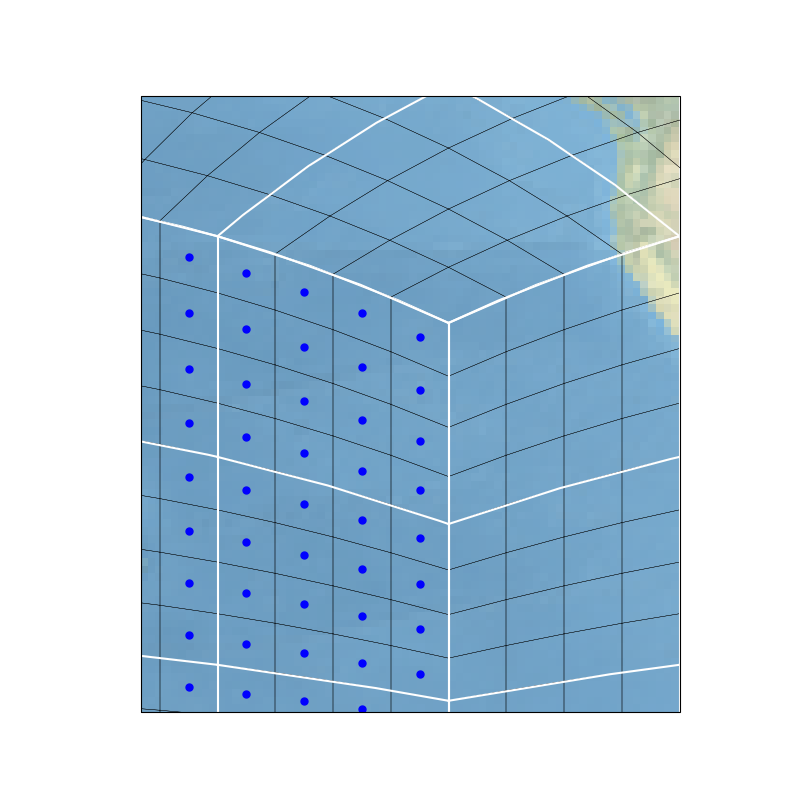
\includegraphics[width=0.8\linewidth]{duoscalar1}
		\caption{A-grid values (blue circles).\label{cs-duoscalar-1}}
	\end{subfigure}
	\begin{subfigure}{0.45\textwidth}
		\centering
		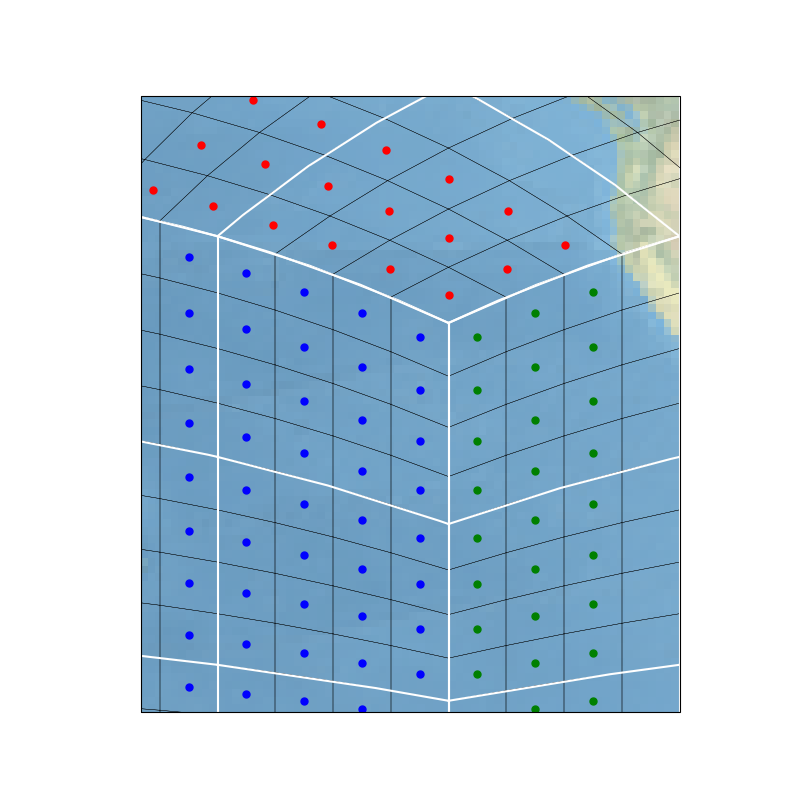
\includegraphics[width=0.8\linewidth]{duoscalar2}
		\caption{Kinked A-grid values (red and green circles)\label{cs-duoscalar-2}}
	\end{subfigure}

	\begin{subfigure}{0.45\textwidth}
		\centering
		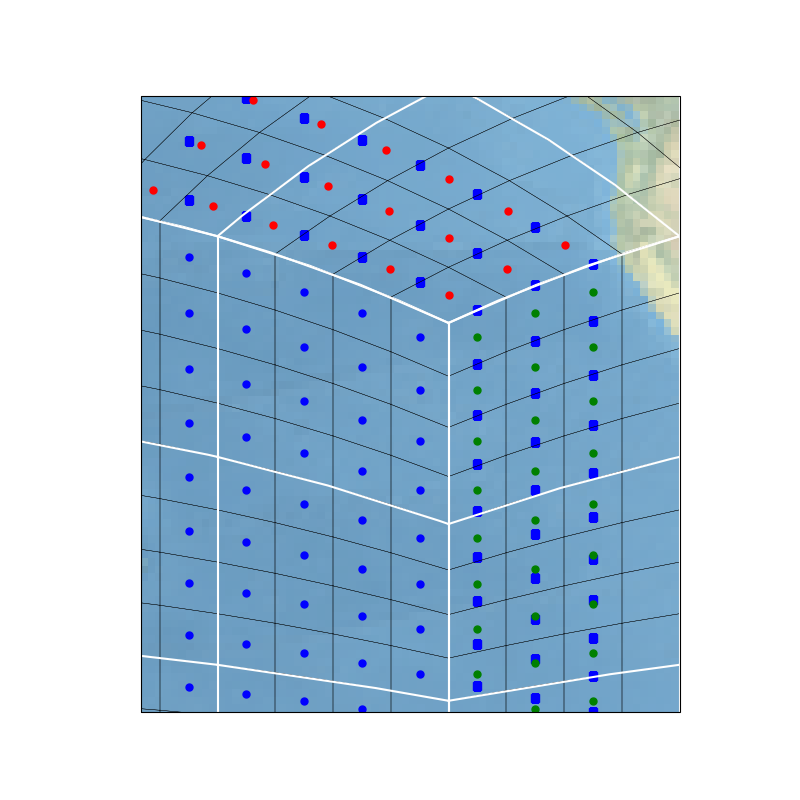
\includegraphics[width=0.8\linewidth]{duoscalar3}
		\caption{A duo-grid points (blue squares)\label{cs-duoscalar-3}}
	\end{subfigure}
	\begin{subfigure}{0.45\textwidth}
	\centering
	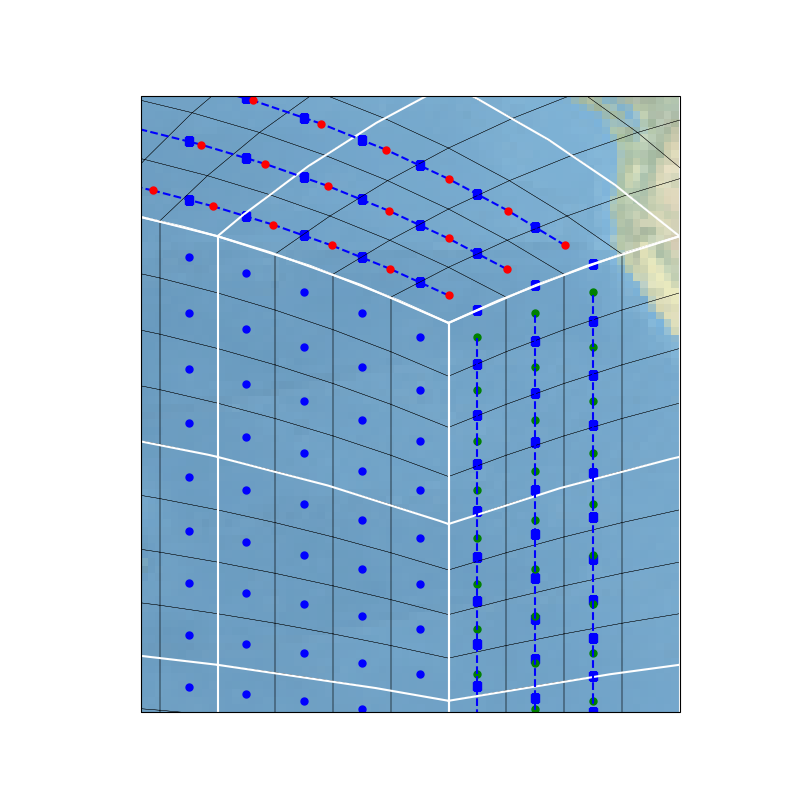
\includegraphics[width=0.8\linewidth]{duoscalar4}
	\caption{Interpolation lines (dashed blue lines)\label{cs-duoscalar-4}}
    \end{subfigure}
 	\caption{Illustration of the A duo-grid interpolation for a scalar field. \label{cs-duoscalar}}
\end{figure}

To illustrate this process in Panel 1, we depict the values of $q_{ijp}$ in Figure \ref{cs-duoscalar}. 
The blue circles represent the values in Panel 1 (Figure \ref{cs-duoscalar-1}), while the red and green circles 
represent the so called \textbf{kinked} values in the other panels (Figure \ref{cs-duoscalar-2}). 
Assuming a halo size of 3, we also indicate the target values at the ghost cell 
positions using blue squares (Figure \ref{cs-duoscalar-3}). 
It is worth noting that the dashed blue lines in Figure \ref{cs-duoscalar-4} 
illustrate how the ghost cell points lie on geodesics containing grid positions from adjacent panels.
With the exception of the blue  squares that lie on a cube corner (Figure \ref{cs-duoscalar-4}),
all the ghost cell values can be obtained using 1D Lagrange interpolation, 
utilizing the surrounding red/green circles on the geodesic. 
This interpolation procedure can be performed for all panels. 
Subsequently, the blue squares that are on a cube corner can be interpolated using the values obtained in the first step of interpolation 
while preserving the order of accuracy of the interpolation, assuming it is fixed.

There are two ways of computing the Lagrange polynomials.
The first one is based on the geodesic distances of the duo-grid line points.
This approach was explored in \citet{chen:2021} and \citet{mouallem:2023}, and we are going to consider it here, calling it \textbf{dg1}.
The second one is to use cube-based distances, where all duo-grid and kinked points are remapped to the plane using the inverse of the cube mapping. 
This approach has the advantage of having uniformly spaced data (the remapped kinked values) used in the duo-grid points interpolation.
This approach is called \textbf{dg2}.
\begin{figure}[!htb]
	\centering
	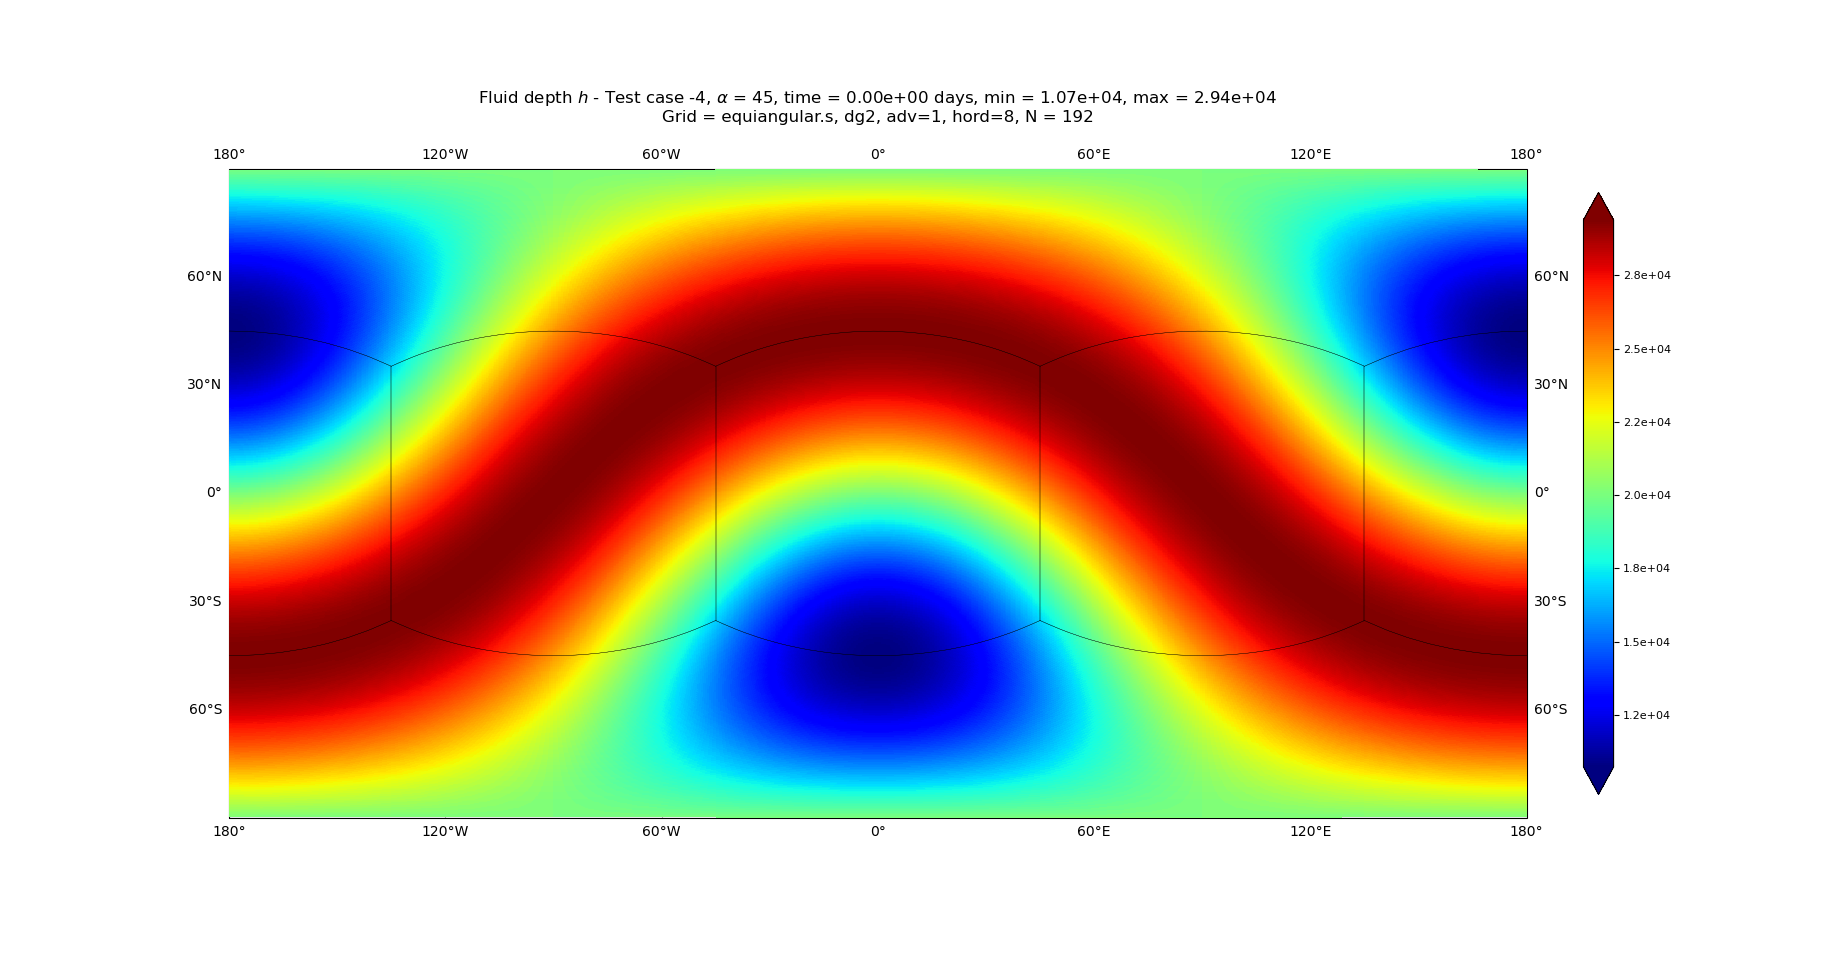
\includegraphics[width=0.8\linewidth]{h_tc-4_t0_alpha45_C192_g2.s_dg2_adv1_hord8_tf12}
	\caption{Scalar field from Equation \eqref{duo-tc1}.\label{cs-duo-tc1}}
\end{figure}

We are going to show a numerical example of this interpolation process using a halo region of size 3 and cubic polynomials.
We shall consider the following trigonometric function
from test case 2 in \citet{will:1992} in our tests:
\begin{equation}
\label{duo-tc1}
q(\lambda, \phi) = h_0 - \frac{1}{g}\bigg(R\Omega u_0 + \frac{u_0^2}{2}\bigg)
\bigg( -\cos(\lambda)\cos(\phi)\sin(\alpha) + \sin(\phi)\cos(\alpha) \bigg)^2,
\end{equation}
where $h_0 = 3\times 10^3 $,
$\alpha=\frac{\pi}{4}$, $u_0 = \frac{2\pi R}{12 \text{days}}$,  $g=9.8$ is the gravity and $\Omega=7.2921 \times 10^{-5}$ is the earth angular rotation speed.
In Figure \ref{cs-duo-tc1} we depict the graph of this field.

We compute the maximum errors for values of $N$ of the form $N=48\times2^k$, where $k$ ranges from 0 to 4. 
We consider g0.s and g0.c, each one with dg1 and dg2, whose errors are depicted in Figure \ref{cs-duoscalar-tc1-g0}.
Additionally, we analyze g2.s and g2.c, each one with dg1 and dg2, and their errors are illustrated in Figure \ref{cs-duoscalar-tc1-g2}.

From the dashed lines in Figure \ref{cs-tc1-error}, we observe that both dg1 and dg2 achieve fourth-order accuracy when the midpoints use the cube formulation, 
with dg2 being much more accurate than dg1.
Both dg1 and dg2 are very similar in this case.
However, when spherical midpoints are employed, we observe a reduction in accuracy by two orders, as indicated by the solid lines.
This discrepancy arises due to a second-order mismatch between cube and spherical midpoints, as discussed in Section \ref{duogrid-points}.
Finally, we observe that the g0 grid yields slightly better results than g2 for cube midpoints formulation.
\begin{figure}[!htb]
	\centering
	\begin{subfigure}{0.45\textwidth}
		\centering
		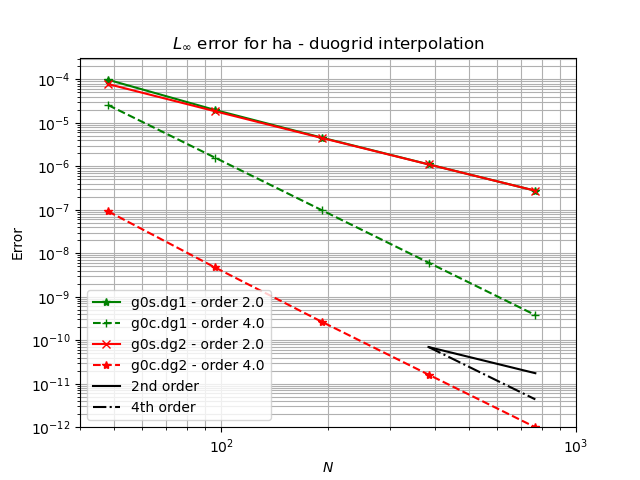
\includegraphics[width=1\linewidth]{g0_duo_error_tc-2_ha}
		\caption{Error for g0.\label{cs-duoscalar-tc1-g0}}
	\end{subfigure}
	\begin{subfigure}{0.45\textwidth}
		\centering
		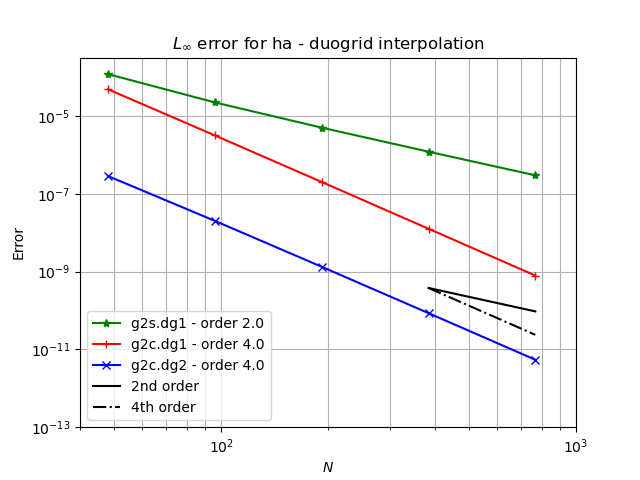
\includegraphics[width=1\linewidth]{g2_duo_error_tc-2_ha}
		\caption{Error for g2.\label{cs-duoscalar-tc1-g2}}
	\end{subfigure}
	\caption{Error for the duo-grid interpolation of the scalar field of \eqref{duo-tc1} for the grid g0 (left) and g2 (right).
Dashed lines use the cube midpoint formulation, while solid lines use the spherical midpoint formulation.
Green lines represent dg1, and red lines represent dg2.\label{cs-tc1-error}}
\end{figure}


\subsection{Ghost cells wind interpolation}
\label{cs-wind-interp}
Let us consider the following problem: Assume that we are given a tangent vector field of the sphere, denoted as 
$\boldsymbol{u}:\mathbb{S}^2_R \to \mathbb{R}^3$. We also have its normal covariant components at the C and D grid points, namely $u_{i+\frac{1}{2},j,p}$ for $i=0, \ldots, N$ and $j=1, \ldots, N$, as well as
$v_{i,j+\frac{1}{2},p}$ for $i=1, \ldots, N$ and $j=0, \ldots, N$. This grid function is called C-grid wind (Figure \ref{cs-duovec-1}).

Our objective is to obtain the values 
\begin{align*}
	u_{i+\frac{1}{2},j,p} \quad \text{ for} \quad &i=-1, \ldots, N+1, \quad &j=-\nu+1, \ldots, 0, \quad &j=N, \ldots, N+\nu,\\
	v_{i,j+\frac{1}{2},p} \quad \text{ for} \quad &j=0, \ldots, N, \quad &i=-\nu+1, \ldots, 0,\quad &i=N, \ldots, N+\nu.
\end{align*}
This problem arises when we apply the dimension splitting method on each panel of the cubed-sphere.
\begin{figure}[!htb]
	\centering
	\begin{subfigure}{0.45\textwidth}
		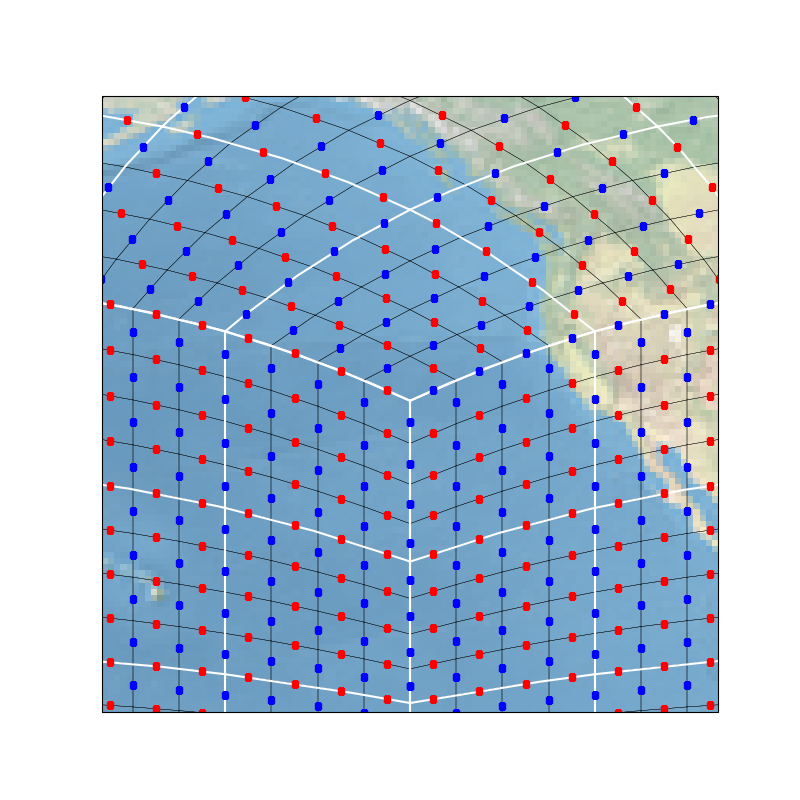
\includegraphics[width=0.8\linewidth]{duowind1}
		\caption{C-grid wind values (blue and red squares).\label{cs-duovec-1}}
	\end{subfigure}
	\begin{subfigure}{0.45\textwidth}
		\centering
		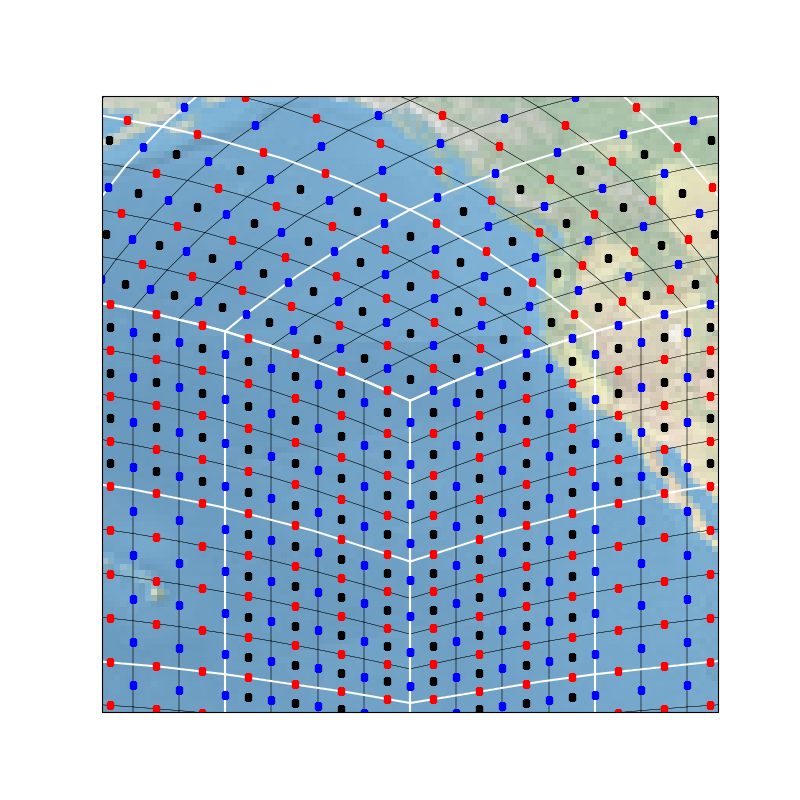
\includegraphics[width=0.8\linewidth]{duowind2}
		\caption{A-grid wind (black circles)\label{cs-duovec-2}}
	\end{subfigure}
	
	\begin{subfigure}{0.45\textwidth}
		\centering
		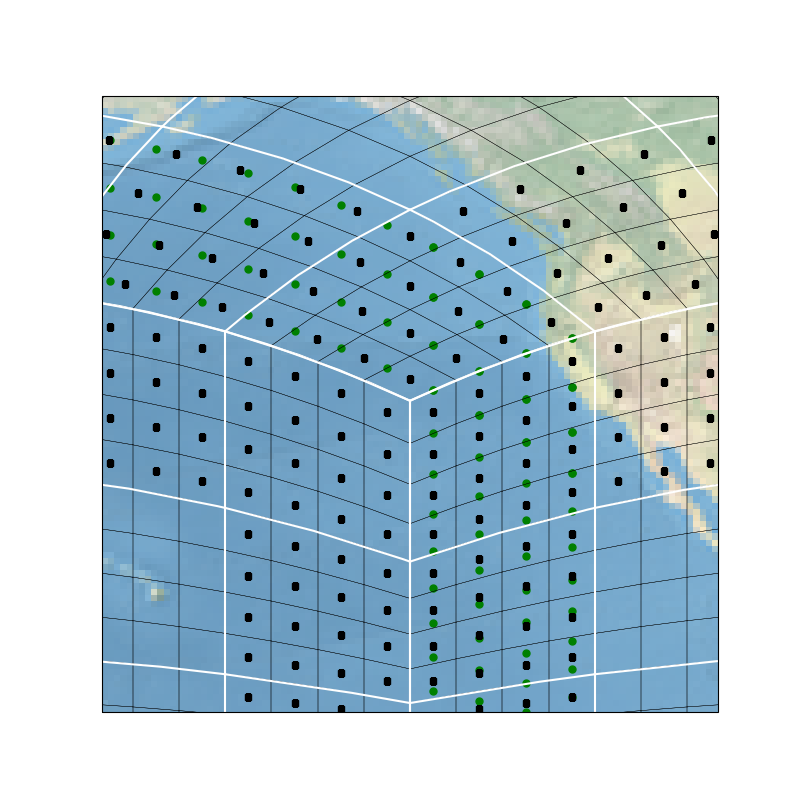
\includegraphics[width=0.8\linewidth]{duowind3}
		\caption{A-duo-grid points (green circles)\label{cs-duovec-3}}
	\end{subfigure}
	\begin{subfigure}{0.45\textwidth}
		\centering
		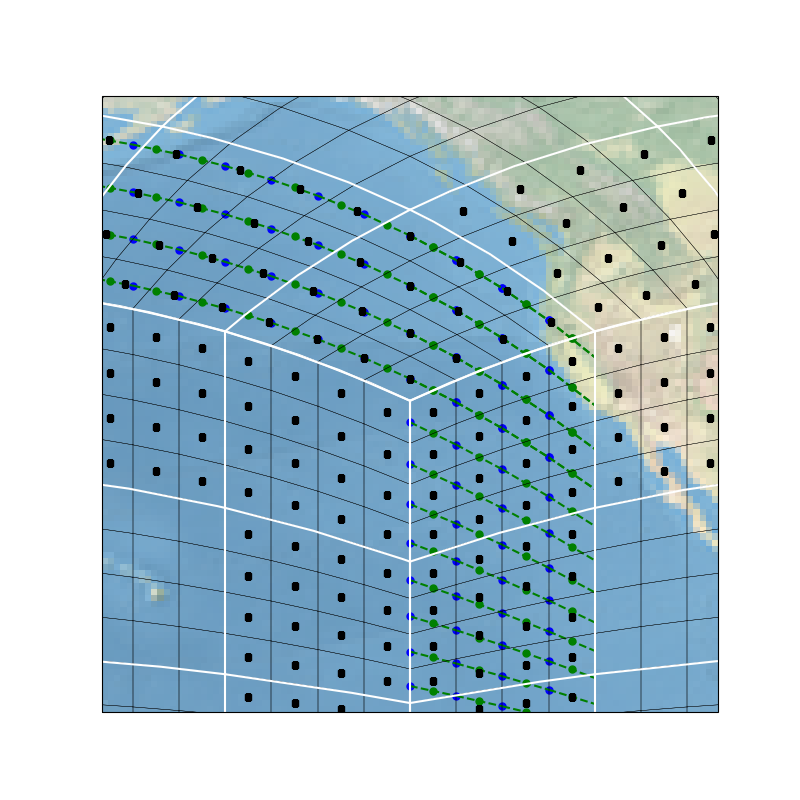
\includegraphics[width=0.8\linewidth]{duowind4}
		\caption{C-duo-grid  wind values (green circles) \label{cs-duovec-4}}
	\end{subfigure}
	\caption{Illustration of the C duo-grid interpolation for a C-grid wind. \label{cs-duovec}}
\end{figure}

This problem can be solved by using the duo-grid interpolation process described earlier for a scalar field.
To apply that interpolation process, we first need to interpolate the values of $u$ and $v$ from the
edges to the A grid points required for the ghost cells interpolation (Figure \ref{cs-duovec-2}).
Specifically, we need the values:
\begin{align*}
	u_{1+k,j,p}, v_{1+k,j,p} \quad \text{ for} \quad &j=1, \ldots, N, \quad k=0, \ldots, \nu,\\
	u_{N-k,j,p}, v_{N-k,j,p} \quad \text{ for} \quad &j=1, \ldots, N, \quad k=0, \ldots, \nu,\\
	u_{i,1+k,p}, v_{i,1+k,p} \quad \text{ for} \quad &i=1, \ldots, N, \quad k=0, \ldots, \nu,\\
	u_{i,N-k,p}, v_{i,N-k,p} \quad \text{ for} \quad &i=1, \ldots, N, \quad k=0, \ldots, \nu.\\
\end{align*}
We apply a simple linear interpolation to remap $u$ and $v$ to the A-grid points (Figure \ref{cs-duovec}). 
However, we are going to use one extra layer of A-grid points since they will be needed for re-interpolation to the C and D grid points
For instance, for 3 layers of ghost cells, we need 4 layers of A duo-grid points as shown in Figure \ref{cs-duovec-2}.
Once these interpolated values are computed, we convert the covariant values $u_{ijp}, v_{ijp}$
to their latitude-longitude components $(u_{\lambda})_{ijp}, (v_{\phi})_{ijp}$ using Equations \eqref{norm-contravariant-to-covariant} and
\eqref{ll-to-normcontravariant}. This conversion avoid any coordinate system discontinuity.
Then, we can use the ghost cell centers interpolation procedure described before for the latitude-longitude components
to recover the wind at the ghost cell centers using any polynomial degree (Figures \ref{cs-duovec-3}).
Finally, we can use the values at the ghost cell centers to obtain the values at the ghost cell edges
by employing a linear interpolation once again (Figures \ref{cs-duovec-4}).
Subsequently, the covariant components can be obtained by using Equations \eqref{ll-to-normcontravariant} and \eqref{norm-contravariant-to-covariant}.

We will consider the following rotated zonal field, as a numerical test, based on \citet{will:1992}:
\begin{align}
	\label{duo-wind1}
	\begin{cases}
		u_\lambda(\lambda,\phi,t) = u_0(\cos(\phi)\cos(\alpha) + \sin(\phi)\cos(\lambda)\sin(\alpha)),\\
		v_\phi(\lambda,\phi,t) = -u_0\sin(\lambda)\sin(\alpha).
	\end{cases}
\end{align}
Here,  $u_0 = \frac{2\pi R}{12 \text{days}}$ and $\alpha= \frac{\pi}{4}$. We will adopt the same grids and schemes as in Section \ref{cs-interp}.
Next, we will compute the relative errors of the covariant components at the midpoint edges.
The errors are presented in Figure \ref{cs-tc2-error}, along with the convergence rate for different degrees employed in the ghost cell center interpolation.
We emphasize that, since we utilize a linear interpolation to retrieve the wind at A-grid from the edges, as well as in the interpolation
from the A duo-grid to C/D duo-grid points, the maximum attainable scheme order is 2.
Indeed, from Figure \ref{cs-tc2-error}, we observe that when employing a cubic polynomials in the duo-grid interpolation step, the final order achieved is 2.
We can also observe again that the spherical midpoints yield larger errors than the cube midpoints formulation.
Additionally, dg2 yields smaller errors, and overall, g0 performs slightly better than g2.
\begin{figure}[!htb]
	\centering
	\begin{subfigure}{0.45\textwidth}
		\centering
		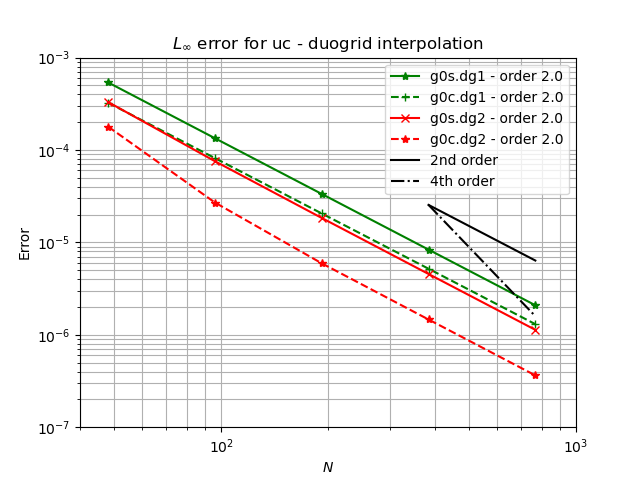
\includegraphics[width=1\linewidth]{g0_duo_error_tc-2_uc}
		\caption{Error for g0.\label{cs-duoscalar-tc2-g0}}
	\end{subfigure}
	\begin{subfigure}{0.45\textwidth}
		\centering
		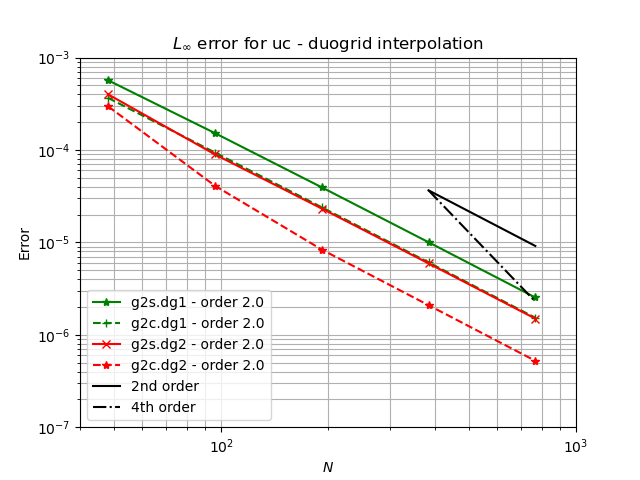
\includegraphics[width=1\linewidth]{g2_duo_error_tc-2_uc}
		\caption{Error for g2.\label{cs-duoscalar-tc2-g2}}
	\end{subfigure}
	\caption{As Figure \ref{cs-tc1-error} but using the C-grid wind given by Equation \eqref{duo-wind1}.\label{cs-tc2-error}}
\end{figure}

\subsection{Edges reconstruction}
\label{cs-recon}
Let us consider the following problem: given the values $q_{ijp}$ we wish to find 
approximations of the function $q$ at the C and D grid points denoted by
\begin{align*}
	q^{L,x}_{ijp}  \approx q_{{i-\frac{1}{2}},j,p},\quad
	q^{R,x}_{ijp}  \approx q_{{i+\frac{1}{2}},j,p},\quad
	q^{L,y}_{ijp}  \approx q_{i,{j-\frac{1}{2}},p},\quad
	q^{R,y}_{ijp}  \approx q_{i,{j+\frac{1}{2}},p}.
\end{align*}

We can estimate the desired values by using the one-dimensional reconstruction schemes 
described in Section \ref{chp-adv1d-sec-recon},
performing PPM reconstruction independently in the $x$ and $y$ directions. 
It is worth noting that all the schemes discussed in those sections are 
expected to be second-order accurate due to the centroid point approximation.

There are  some differences in the computation of the stencil near the cube edges.
Unlike in the previous chapters, where periodic boundary conditions were assumed, 
the boundary conditions in this context are related to the adjacent panels. 
One way to address this issue is to use the duo-grid as discussed  in Section \ref{cs-interp} to compute the stencils. 
We are going to consider the dg2 method, since it yields better results overall.

Another approach, employed in \citet{sadourny:1972}, involves ignoring the
discontinuity of the coordinate system and simply using the values of the cells 
in the adjacent panels as the ghost cell values. 
Additionally, an alternative method that avoids the use of ghost cells was developed by
\citet{putman:2007}, which entails extrapolation at the cells surrounding the cube edge.
We will refer to this scheme as \textbf{kinked} method.
This scheme uses the following extrapolations:
\begin{align*}
	q^{L,x}_{1,j,p} &= \frac{1}{2}\bigg(3Q_{1,j,p} - Q_{2,j,p}\bigg),\\
	q^{R,x}_{N,j,p} &= \frac{1}{2}\bigg(3Q_{N,j,p} - Q_{N-1,j,p}\bigg),
\end{align*}
at the points that are located on the cube edges. The other edge values are estimated as:
\begin{align*}
	q^{R,x}_{1,j,p} &= \frac{1}{14}\bigg(3Q_{1,j,p} + 11Q_{2,j,p} - 2(Q_{3,j,p} - Q_{1,j,p})\bigg),\\
	q^{L,x}_{2,j,p} &= q^{R,x}_{1,j,p},\\
	q^{L,x}_{N,j,p} &= \frac{1}{14}\bigg(3Q_{N,j,p} + 11Q_{N-1,j,p} - 2(Q_{N-2,j,p} - Q_{N,j,p})\bigg),\\
	q^{R,x}_{N-1,j,p} &= q^{L,x}_{N,j,p},\\
\end{align*}
in the $x$ direction. Similar formulas are used in the $y$ direction.
We are going to use the trigonometric function (Equation \eqref{duo-tc1})
as before on the unit sphere to compare the schemes kinked and dg2. The scheme dg2 uses cubic polynomials.
We introduce the relative errors:
\begin{align*}
	e_{{i-\frac{1}{2}},j,p} &= (|q_{{i-\frac{1}{2}},j,p} - q^{L,x}_{ijp}|)/|q_{{i-\frac{1}{2}},j,p}|,\\
	e_{{i+\frac{1}{2}},j,p} &= (|q_{{i+\frac{1}{2}},j,p} - q^{R,x}_{ijp}|)/|q_{{i+\frac{1}{2}},j,p}|,\\
	e_{i,{j-\frac{1}{2}},p} &= (|q_{i,{j-\frac{1}{2}},p} - q^{L,y}_{ijp}|)/|q_{i,{j-\frac{1}{2}},p}|,\\
	e_{i,{j+\frac{1}{2}},p} &= (|q_{i,{j+\frac{1}{2}},p} - q^{R,y}_{ijp}|)/|q_{i,{j+\frac{1}{2}},p}|,\\
	e_{ijp} &= \max\{e_{{i-\frac{1}{2}},j,p}, e_{{i+\frac{1}{2}},j,p} , e_{i,{j-\frac{1}{2}},p}, e_{i,{j+\frac{1}{2}},p} \},\\
	E &= \max \{e_{ijp}\}.
\end{align*}
We are going to compute $E$ for different values of $N$ and different schemes as in the numerical experiments of Section \ref{cs-interp}.

\begin{figure}[!htb]
	\centering
	\begin{subfigure}{0.45\textwidth}
		\centering
		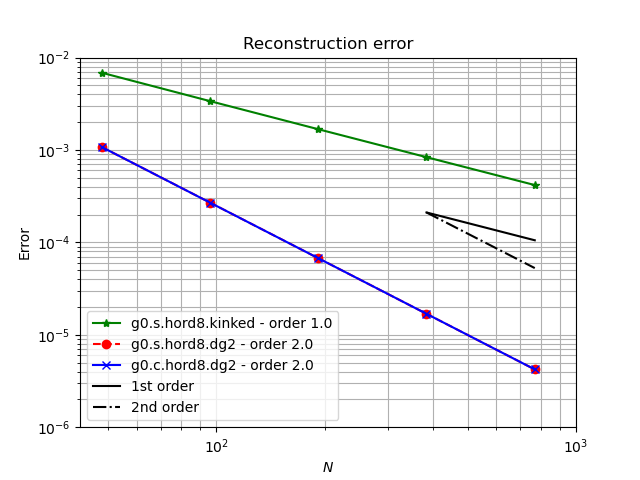
\includegraphics[width=1\linewidth]{hord8_recon_g0.c}
		\caption{Error for g0.\label{cs-recon-g0}}
	\end{subfigure}
	\begin{subfigure}{0.45\textwidth}
		\centering
		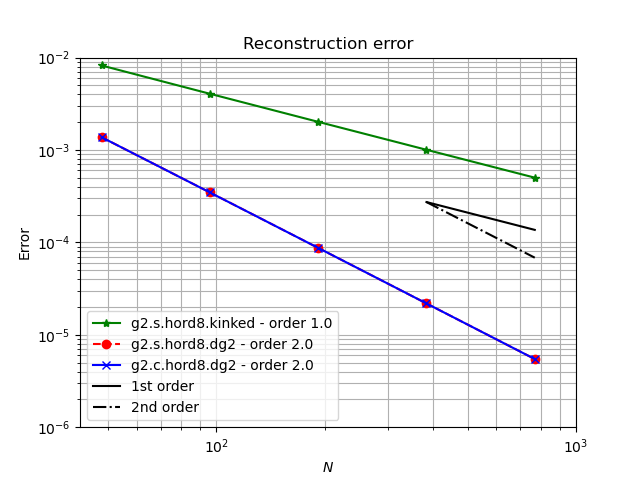
\includegraphics[width=1\linewidth]{hord8_recon_g2.c}
		\caption{Error for g2.\label{cs-recon-g2}}
	\end{subfigure}
	\caption{As Figure \ref{cs-tc1-error} but using the C-grid wind given by Equation \eqref{duo-wind1}.\label{cs-recon-error}}
\end{figure}

\section{Concluding remarks}
\label{cs-conc}

\newpage
\begin{figure}[!htb]
	\centering
	\begin{subfigure}{0.9\textwidth}
		\centering
		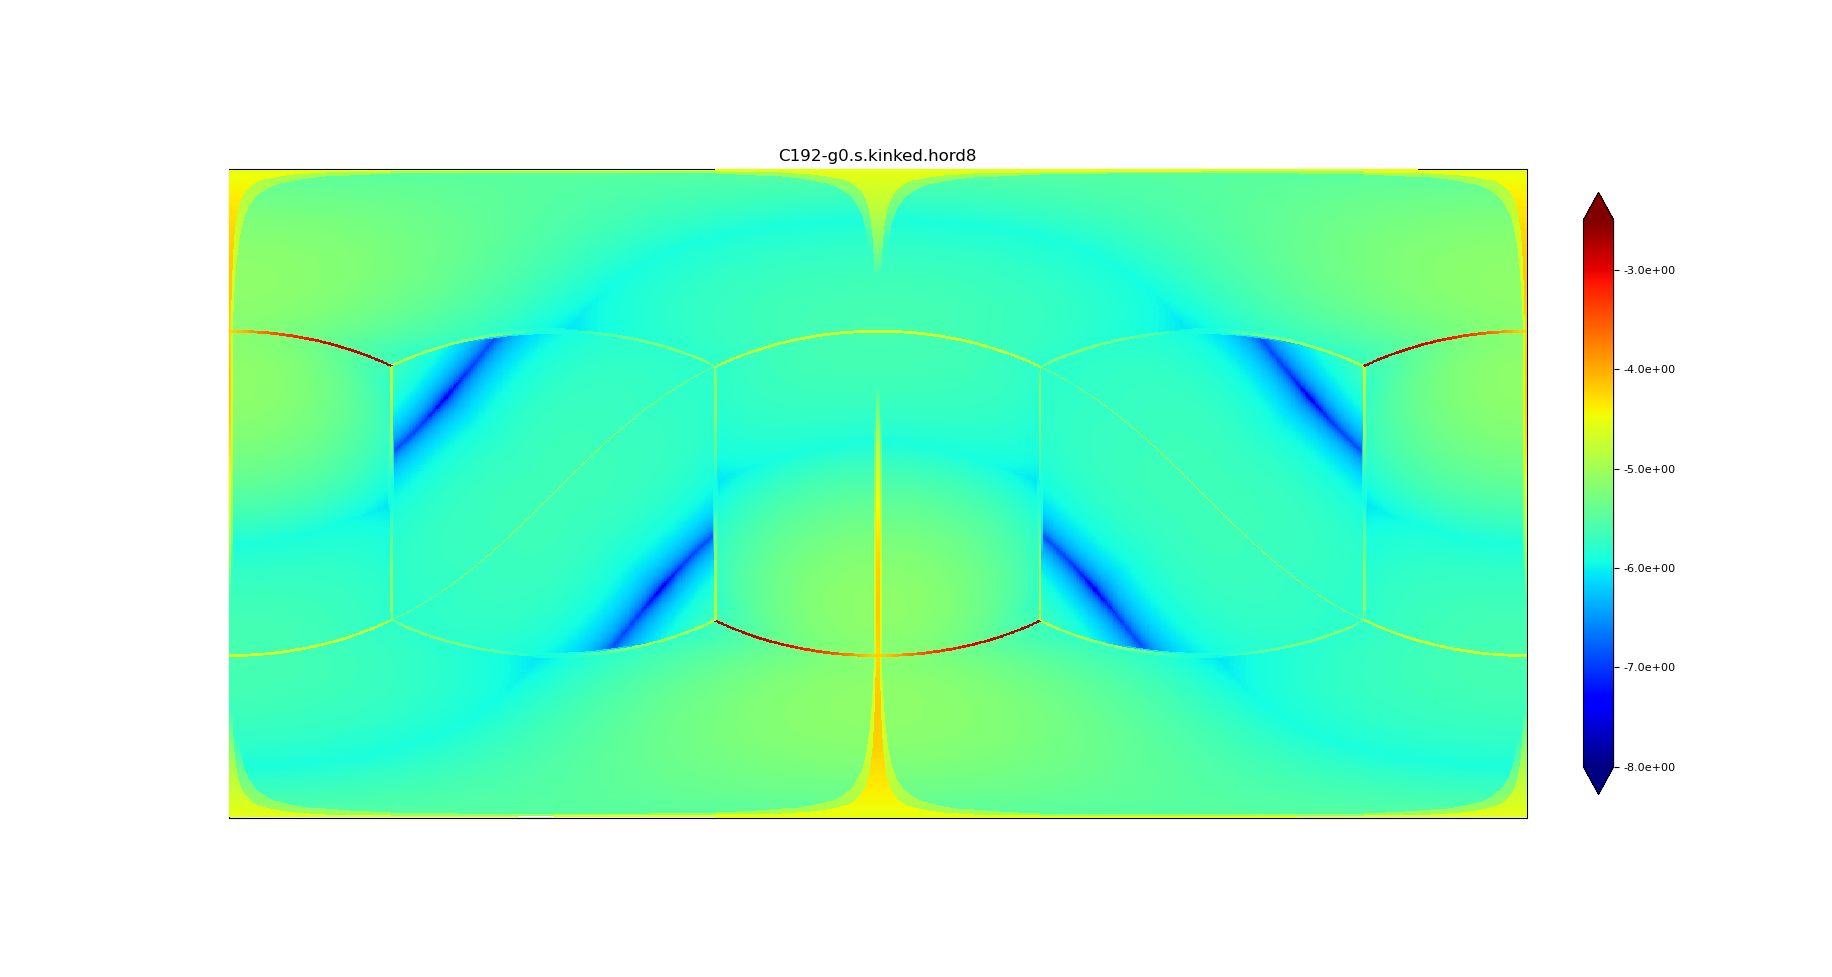
\includegraphics[width=1\linewidth]{recon_g0_192.s.kinked.hord8}
		\caption{g0 grid areas (km$^2$).}
	\end{subfigure}
	
	\begin{subfigure}{0.9\textwidth}
		\centering
		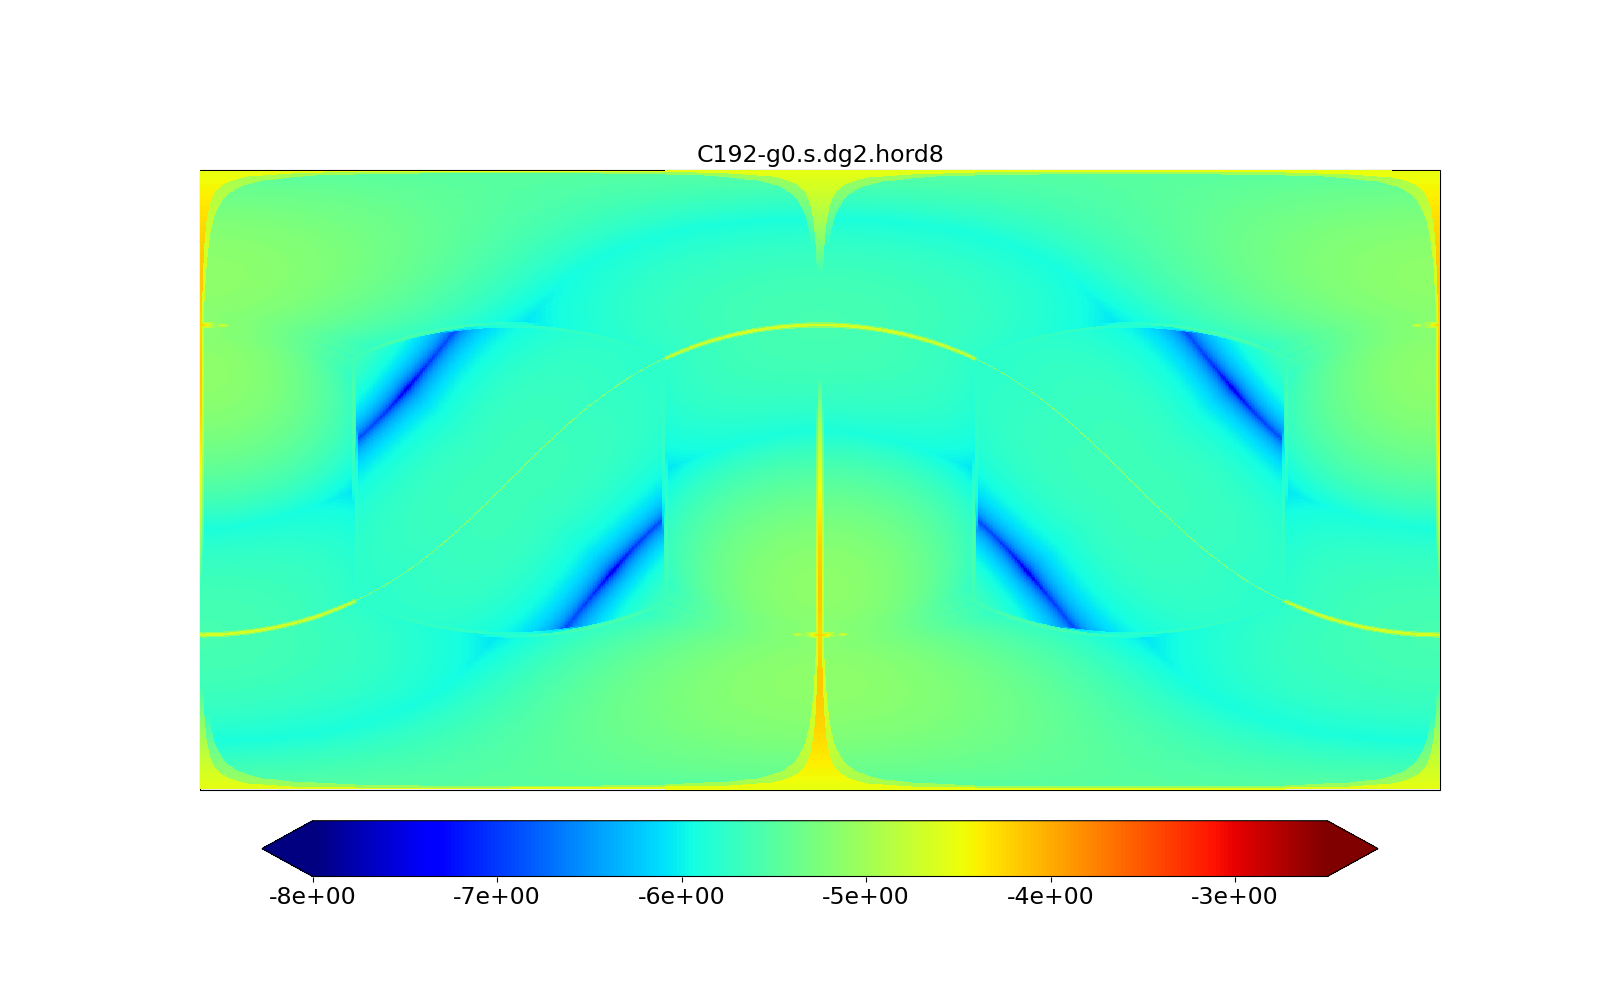
\includegraphics[width=1\linewidth]{recon_g0_192.s.dg2.hord8}
		\caption{g2 grid areas (km$^2$).}
	\end{subfigure}
	
	\begin{subfigure}{0.9\textwidth}
		\centering
		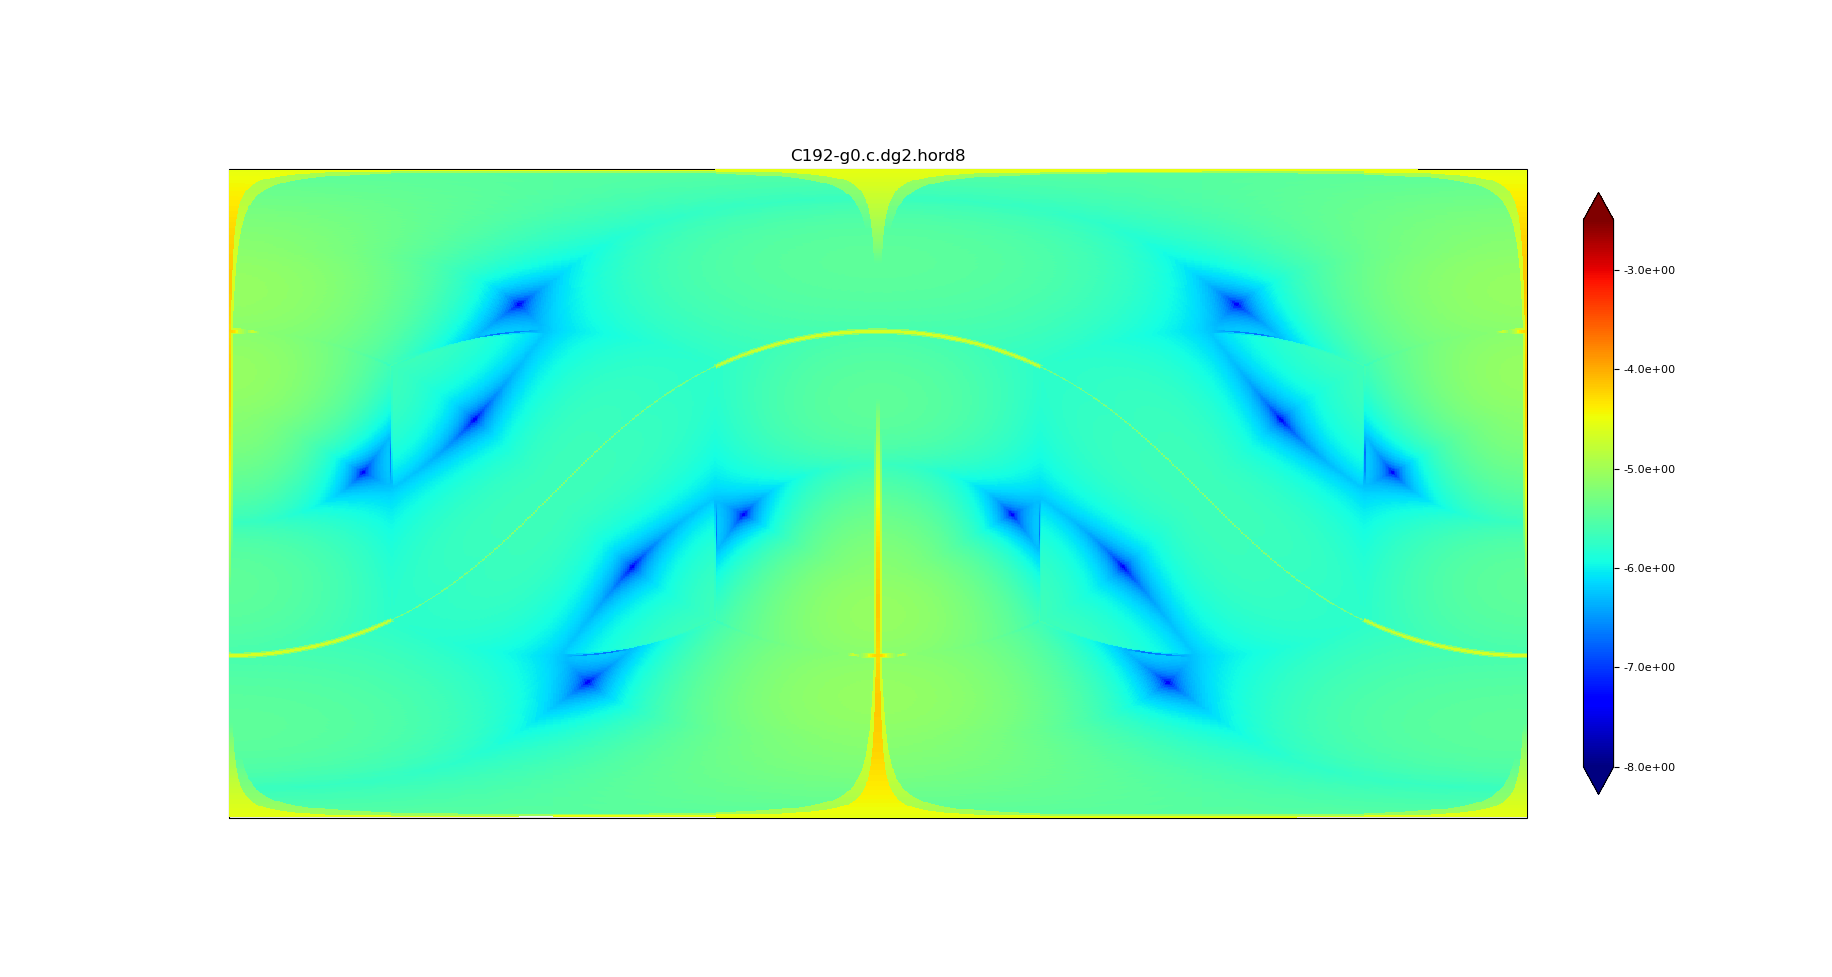
\includegraphics[width=1\linewidth]{recon_g0_192.c.dg2.hord8}
		\caption{g2 grid areas (km$^2$).}
	\end{subfigure}
	\caption{Areas for the grid g0 and g2 using $N=384$.\label{cs-recon-errors-g0}}
\end{figure}

\newpage
\begin{figure}[!htb]
	\centering
	\begin{subfigure}{0.9\textwidth}
		\centering
		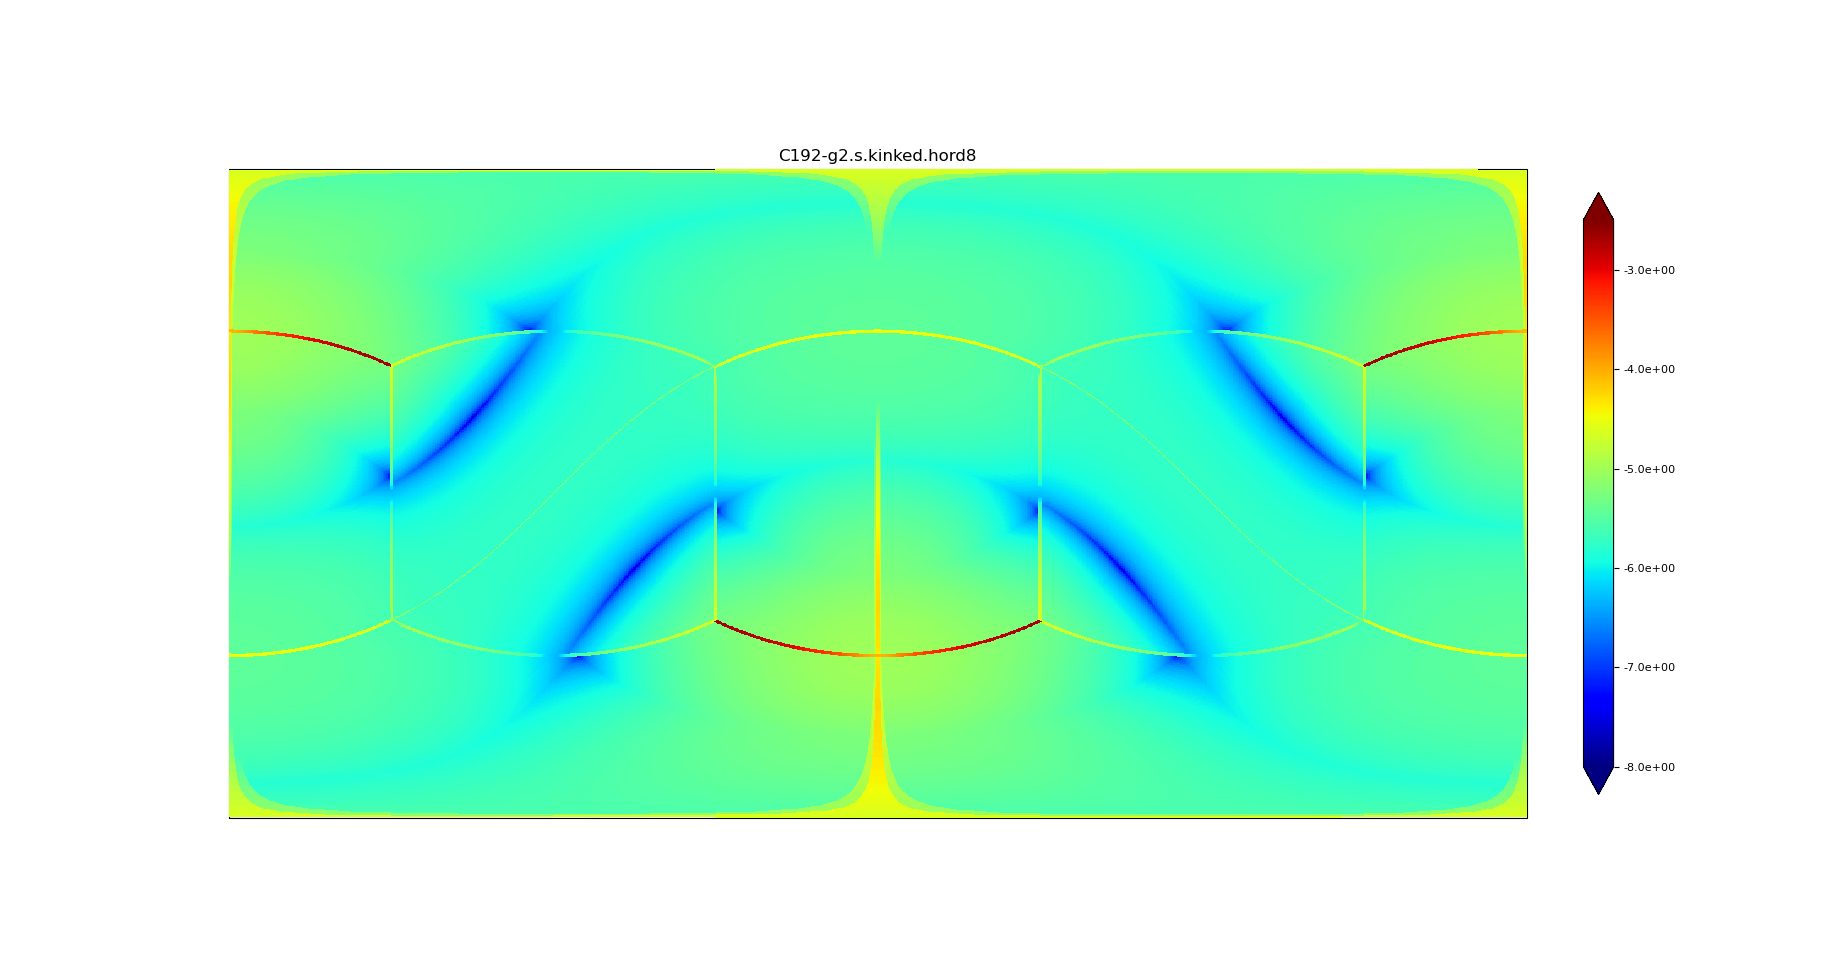
\includegraphics[width=1\linewidth]{recon_g2_192.s.kinked.hord8}
		\caption{g0 grid areas (km$^2$).}
	\end{subfigure}
	
	\begin{subfigure}{0.9\textwidth}
		\centering
		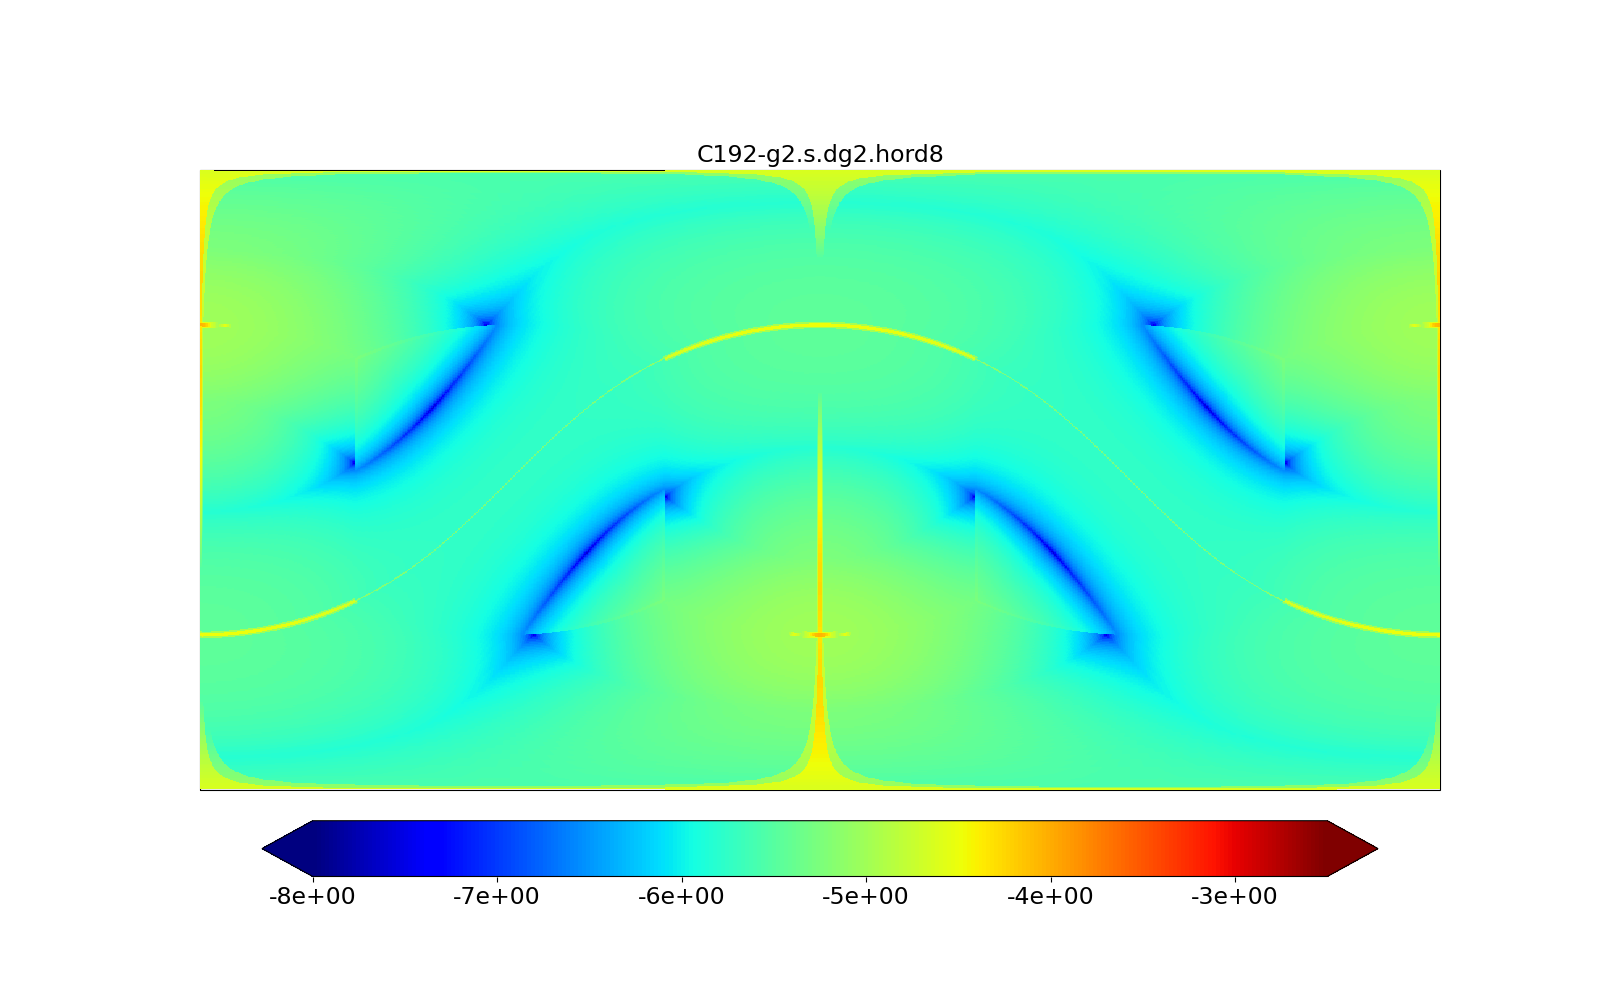
\includegraphics[width=1\linewidth]{recon_g2_192.s.dg2.hord8}
		\caption{g2 grid areas (km$^2$).}
	\end{subfigure}
	
	\begin{subfigure}{0.9\textwidth}
		\centering
		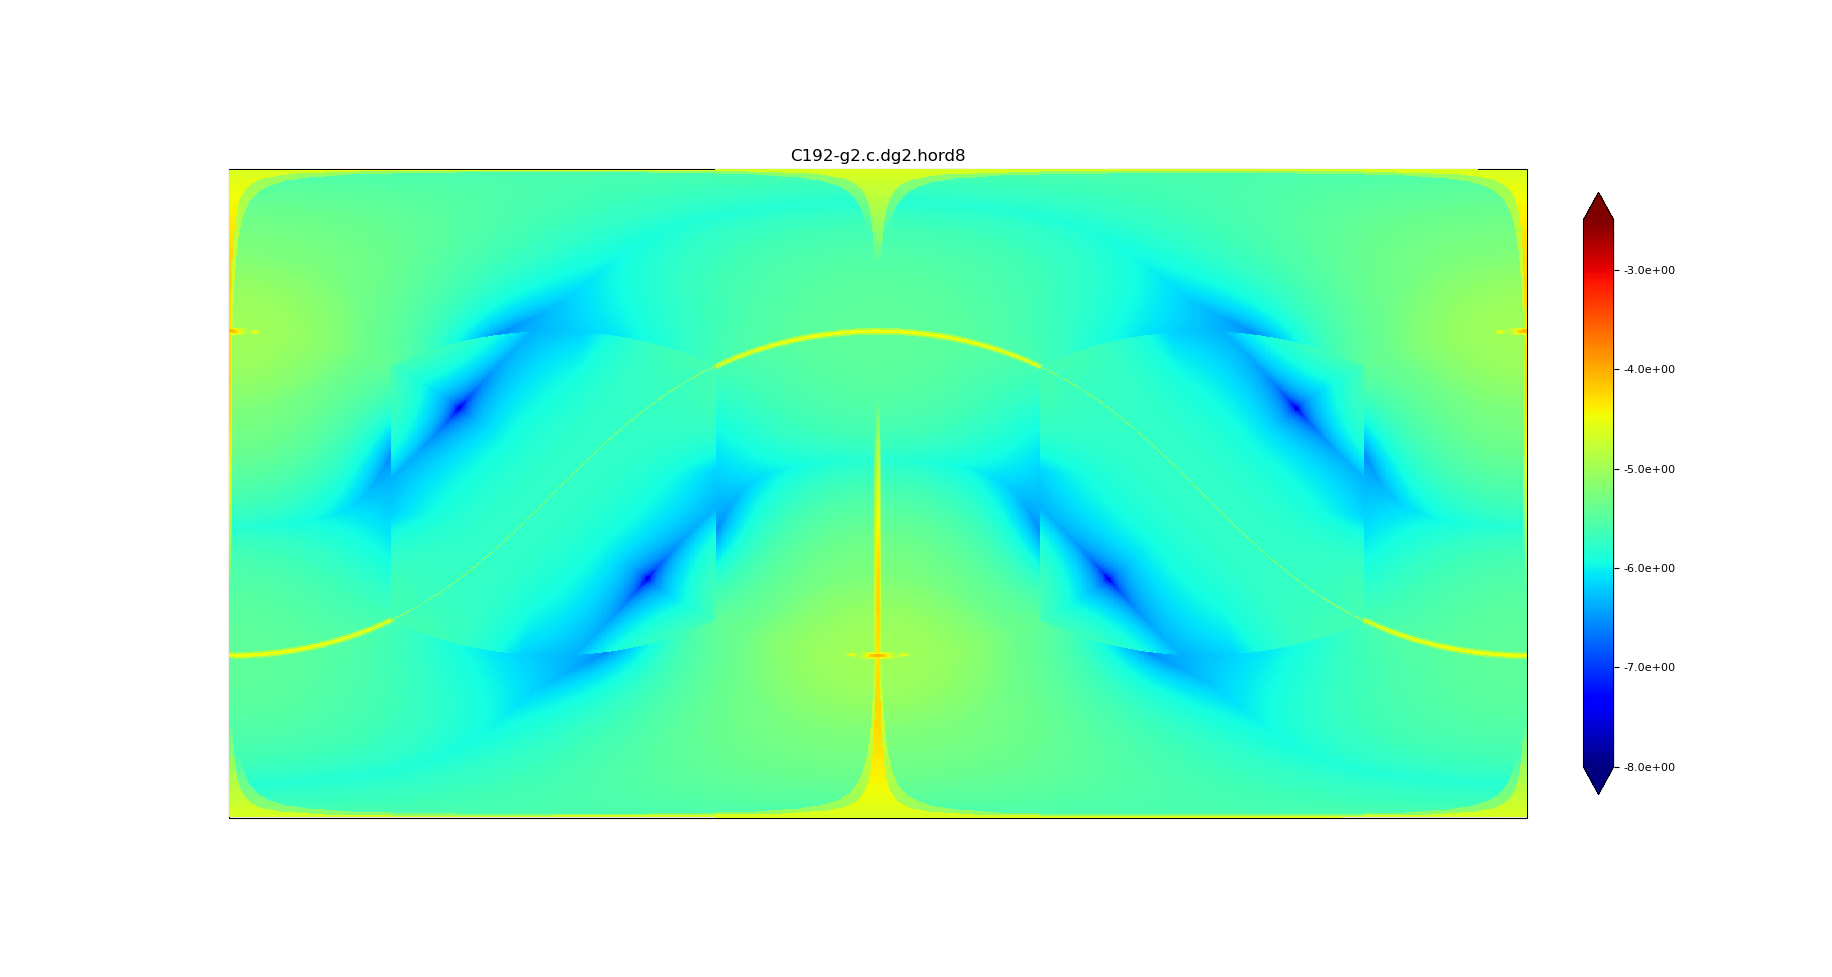
\includegraphics[width=1\linewidth]{recon_g2_192.c.dg2.hord8}
		\caption{g2 grid areas (km$^2$).}
	\end{subfigure}
	\caption{Areas for the grid g0 and g2 using $N=384$.\label{cs-recon-errors-g2}}
\end{figure}



